%! TeX program=latexmk
%! TeX options=-xelatex -synctex=1 -interaction=nonstopmode -file-line-error "%DOC%"
\documentclass[a4paper, nosysfonts]{hpcchina}

\usepackage{graphicx}
\usepackage{amsmath,amsthm}
\usepackage{amssymb,amsfonts}
%以下宏包为测试用途
\usepackage{blindtext}
\usepackage{zhlipsum}
\usepackage{tikz}
\usepackage{metalogo}

%LXN
\graphicspath{ {pictures/} }  %使用图片
\usepackage{algorithm}  % 伪代码编辑
\usepackage{algorithmic}  % 伪代码编辑
\renewcommand{\algorithmicrequire}{\textbf{Input:}}  % 伪代码输入
\renewcommand{\algorithmicensure}{\textbf{Output:}}  % 伪代码输出
\usepackage{setspace}  % 伪代码行距

%标题
\title{基于张量交换和张量重算的大模型推理内存优化技术}

%作者
\author{段晓辉\textsuperscript{1}}
%单位
\affiliation{
  \textsuperscript{1} 清华大学,北京 100084
}
%邮箱,使用\mailurl{地址}可以生成可点击的链接
\email{\mailurl{sunrise_duan@126.com}}

%中文摘要
\cabstract{
大语言模型(LLM)拥有极高的参数量,为推理任务的高效运行带来巨大挑战。传统的LLM推理框架引入了张量交换和张量重算等技术,在有限的GPU内存上以牺牲性能为代价完成LLM推理。然而,已有研究工作无法根据推理任务运行时信息自适应地选择内存优化技术,导致推理任务的性能无法得到进一步提升;同时这些工作没有实现整体吞吐率与单请求延时之间的权衡,仅能以二者之一作为优化目标。针对以上问题,本文面向大模型推理服务场景,提出了一款基于张量交换和张量重算的LLM推理框架。该框架首先实现了张量重算和张量交换开销预测,其预测误差分别在2\%和5\%以下。另外,该框架引入了基于开销感知的张量优化策略,旨在实现面向服务器端的处理加速;同时引入了基于公平性的用户请求调度策略,旨在实现面向客户端的实时请求处理。本文在常见LLM和推理数据集上开展实验。结果表明,基于开销感知的张量优化策略能够为推理任务带来1.2到1.4的整体吞吐加速比;基于公平性的用户请求调度策略能够大幅降低平均带权周转时间。由此证明本文在优化过程中权衡整体吞吐率与单请求延时,化解了二者在实现上的冲突,实现LLM高效推理。
}
%中文关键词
\keyword{
  关键词:大语言模型、推理、张量交换、张量重算
}

%英文标题
\etitle{DeepFake of HPC China Template in \XeLaTeX}
%英文作者
\eauthor{Xiaohui Duan\textsuperscript{1}}
%英文单位
\eaffiliation{
  \textsuperscript{1} (Tsinghua University, Beijing 100084)
}
%英文摘要
\eabstract{
  Large Language Models(LLMs) come with an extremely high amount of parameters, posing significant challenges for inference tasks. Traditional LLM inference services employs swapping and re-computation techniques, guaranteeing the success of the inference tasks at the cost of throughput on limited GPU memory. However, existing LLM serving systems fails to search memory management schemes adaptively based on the runtime information of LLM inference tasks, leading to a sub-optimal performance. And at the same time, these works are inferior in holding a balance between inference throughput and request latency, targeting at only one in these two objectives in the experiments and neglecting the other.To address the above issues, this work presents an adaptive LLM service for inference tasks based on swapping and re-computation technique. Fundamentally, we implement an overhead predictor for swapping and re-computation, with an error rate lower than 2\% and 5\% respectively. Moreover, we develop a cost-aware memory optimization method and a fairness-based request scheduling algorithm. The former speeds the inference task on the server, and the latter improves the real-time performance by reducing request latency targeting at the client. We conduct experiments on typical LLMs and datasets. As a result, the cost-aware memory optimization method accelerates the inference task by 1.2 to 1.4, and the fairness-based request scheduling algorithm can significantly reduce the average weighted around time. This demonstrates that the proposed service makes a better trade off between inference throughput and request latency by resolving their discrepancy in implementation, and achieves efficient LLM inference.
}
%英文关键词
\ekeyword{
  LLM, inference, swapping, re-computation
}

%基金号
\grants{目前无人捐助此项目}
%DOI号
\doi{missing DOI}
%分类号
\clcls{TP391}
%卷(期):起止页,年
\issue{卷(期):起止页,年}
%收稿日期
\dateaccept{yyyy-mm-dd}
%修回日期
\daterevise{yyyy-mm-dd}

\begin{document}
    
\maketitle

\section{引言}
从人脸识别、个性化推荐、到智能家居、无人驾驶等应用领域,深度学习(Deep Learning,DL)相关技术已经融入到社会的方方面面,为人类的生产生活带来了极大的便利。自然语言处理(Natural Language Processing,NLP)作为深度学习领域的重要研究方向,长期以来备受人们关注。近年来,随着GPU算力的不断提升,各种语言模型也朝着复杂化,多功能化的方向迅猛发展。 \par
大语言模型(Large Language Models,LLM)是自然语言处理领域的一个分支。LLM通常拥有十亿级别,甚至万亿级别的参数量,因此需要海量的文本数据进行训练。同时,LLM在多种类型的任务中展现出卓越性能,如文本摘要、机器翻译、代码生成以及对话问答等,拥有巨大的科研价值与商业价值。2021年GPT-3模型的问世标志着LLM领域的里程碑,自此,各大科研机构纷纷投入到相关研究中,各种LLM层出不穷,使得该领域的热度空前高涨。 \par
复杂的结构和爆炸式增长的参数量为LLM带来了卓越的NLP性能,但却为众多的科研工作者们带来了巨大难关。LLM在训练时消耗资源多,花费时间长,失败风险高,性能要求严,使得LLM的训练成本急剧上涨。推理任务的成本相对较低,但极高的内存占用也为推理任务的高效执行带来了独特的挑战。例如,GPT-175B模型仅在权重加载环节就需要消耗325GB的GPU内存空间 ,在传统的LLM推理框架下,需要使用至少5个NVIDIA A100 GPU(80GB),且需要引入复杂的并行化策略。为了应对较高参数量带来的GPU内存瓶颈,本文提出了一款基于张量交换(Swapping)和张量重算(Recomputation)的LLM推理服务框架,引入先进的显存优化策略和用户请求调度策略实现LLM的高效推理。该框架针对服务器端实现高吞吐,针对用户端实现实时请求处理,进一步解决吞吐率与单请求延时在性能优化上长期以来存在的矛盾。 \par
传统的LLM推理框架拥有诸多可改进之处,下面列举其中最为显著的两点。 \par
首先,通过张量交换和张量重算等内存优化技术,可以在有限的GPU内存空间中增加批处理大小。然而,上述两项张量优化技术对LLM推理性能的影响十分复杂,取决于服务器硬件环境(如GPU计算能力、GPU-CPU传输带宽)、用户设置(如新token的采样方式)、LLM与数据集选取、以及推理任务的运行时信息等等。已有的推理框架在面对GPU内存瓶颈时固定调用张量交换或张量重算技术,而无法根据其次、在针对LLM推理任务进行性能优化时,传统工作或者以整体吞吐率为单一导向,或者以单请求延时为单一导向,而没有在二者间进行权衡。吞吐率是面向服务器端的性能优化指标,体现了服务器端的处理效率;单请求平均延时是面向客户端的性能优化指标,体现了用户请求处理的实时性。二者均在LLM应用程序中占有重要地位。 \par
针对传统工作的不足之处,本文设计了一款基于张量交换和张量重算的LLM推理服务框架。具体而言,本文拥有以下贡献:
\begin{itemize}
  \item 本文设计了一款张量重算分析器,实现张量重算的开销预测。通过算子粒度的计算复杂度分析来找出张量重算开销的影响因素,而后模拟LLM的前向传播,收集数据,并建立单步迭代执行时间的回归预测模型。实验表明,张量重算开销预测的误差在2\%以内。
  \item 本文设计了一款张量交换分析器,实现张量交换的开销预测。通过获取用户请求KV Cache的内存占用和GPU-CPU间的通信效率,来计算数据传输开销。实验证明,张量交换开销预测的误差在5\%以内。
  \item 本文设计了一种基于张量交换和张量重算的自适应LLM推理优化器。通过引入基于开销感知的张量优化策略,提升整体吞吐率,实现了面向服务器端的处理加速;通过引入基于公平性的用户请求调度策略,降低单请求平均延时,实现了面向客户端的实时请求处理。
  \item 本文搭建了一款LLM推理服务框架进行实验评估。该框架实现了上述设计的张量重算分析器、张量交换分析器与自适应LLM推理优化器等功能模块。以vLLM框架作为基础程序,在典型LLM(OPT、Llama)和数据集(Writing、Chatbot、Alpaca)上进行实验验证。结果表明,本文能够实现17\%到27\%的吞吐率提升,且大幅度降低用户请求的平均带权周转。以此证明本文的优化技术实现了整体吞吐率与单请求延时的权衡,完成了LLM的高效推理。
\end{itemize}

\section{背景知识}
本章介绍有关KV Cache的背景知识。第一节介绍KV Cache在LLM推理任务中的功能;第二节介绍KV Cache在优化过程中面临的挑战。本文提出的自适应LLM推理优化器主要针对KV Cache进行内存优化。

\subsection{KV Cache的提出}
LLM推理任务的输入与输出均为文本序列。LLM分词器将用户输入文本序列编码成输入token序列,通过LLM推理计算生成输出token序列,最后通过分词器解码生成输出文本序列返回给用户。LLM生成式推理任务采用自回归式解码机制,整个解码过程包含多次前向传播操作(也称迭代),每次迭代仅生成一个新token。 \par
LLM生成式推理任务包含两个阶段:prefill阶段读取用户输入的token序列,生成第一个token;decode阶段分为多步进行,依次生成后续token,直至得到终止token。在推理过程中,每个token拥有一个key-value张量对,实质是其在自注意力机制下的编码结果。 \par
在decode阶段中,每个token的计算均依赖于前序token的key值和value值。如果每次计算前都重新调用自注意力机制来获取前序token的key-value张量,则会产生大量不必要的时间开销。主流LLM推理服务框架普遍采用KV Cache数据结构来保存这些token的key-value张量,方便后续token的生成,避免重复计算,其工作原理如图\ref{KV Cache的功能示意图}所示。
\begin{figure}[!htbp]
  \renewcommand{\arraystretch}{1}
  \centering
  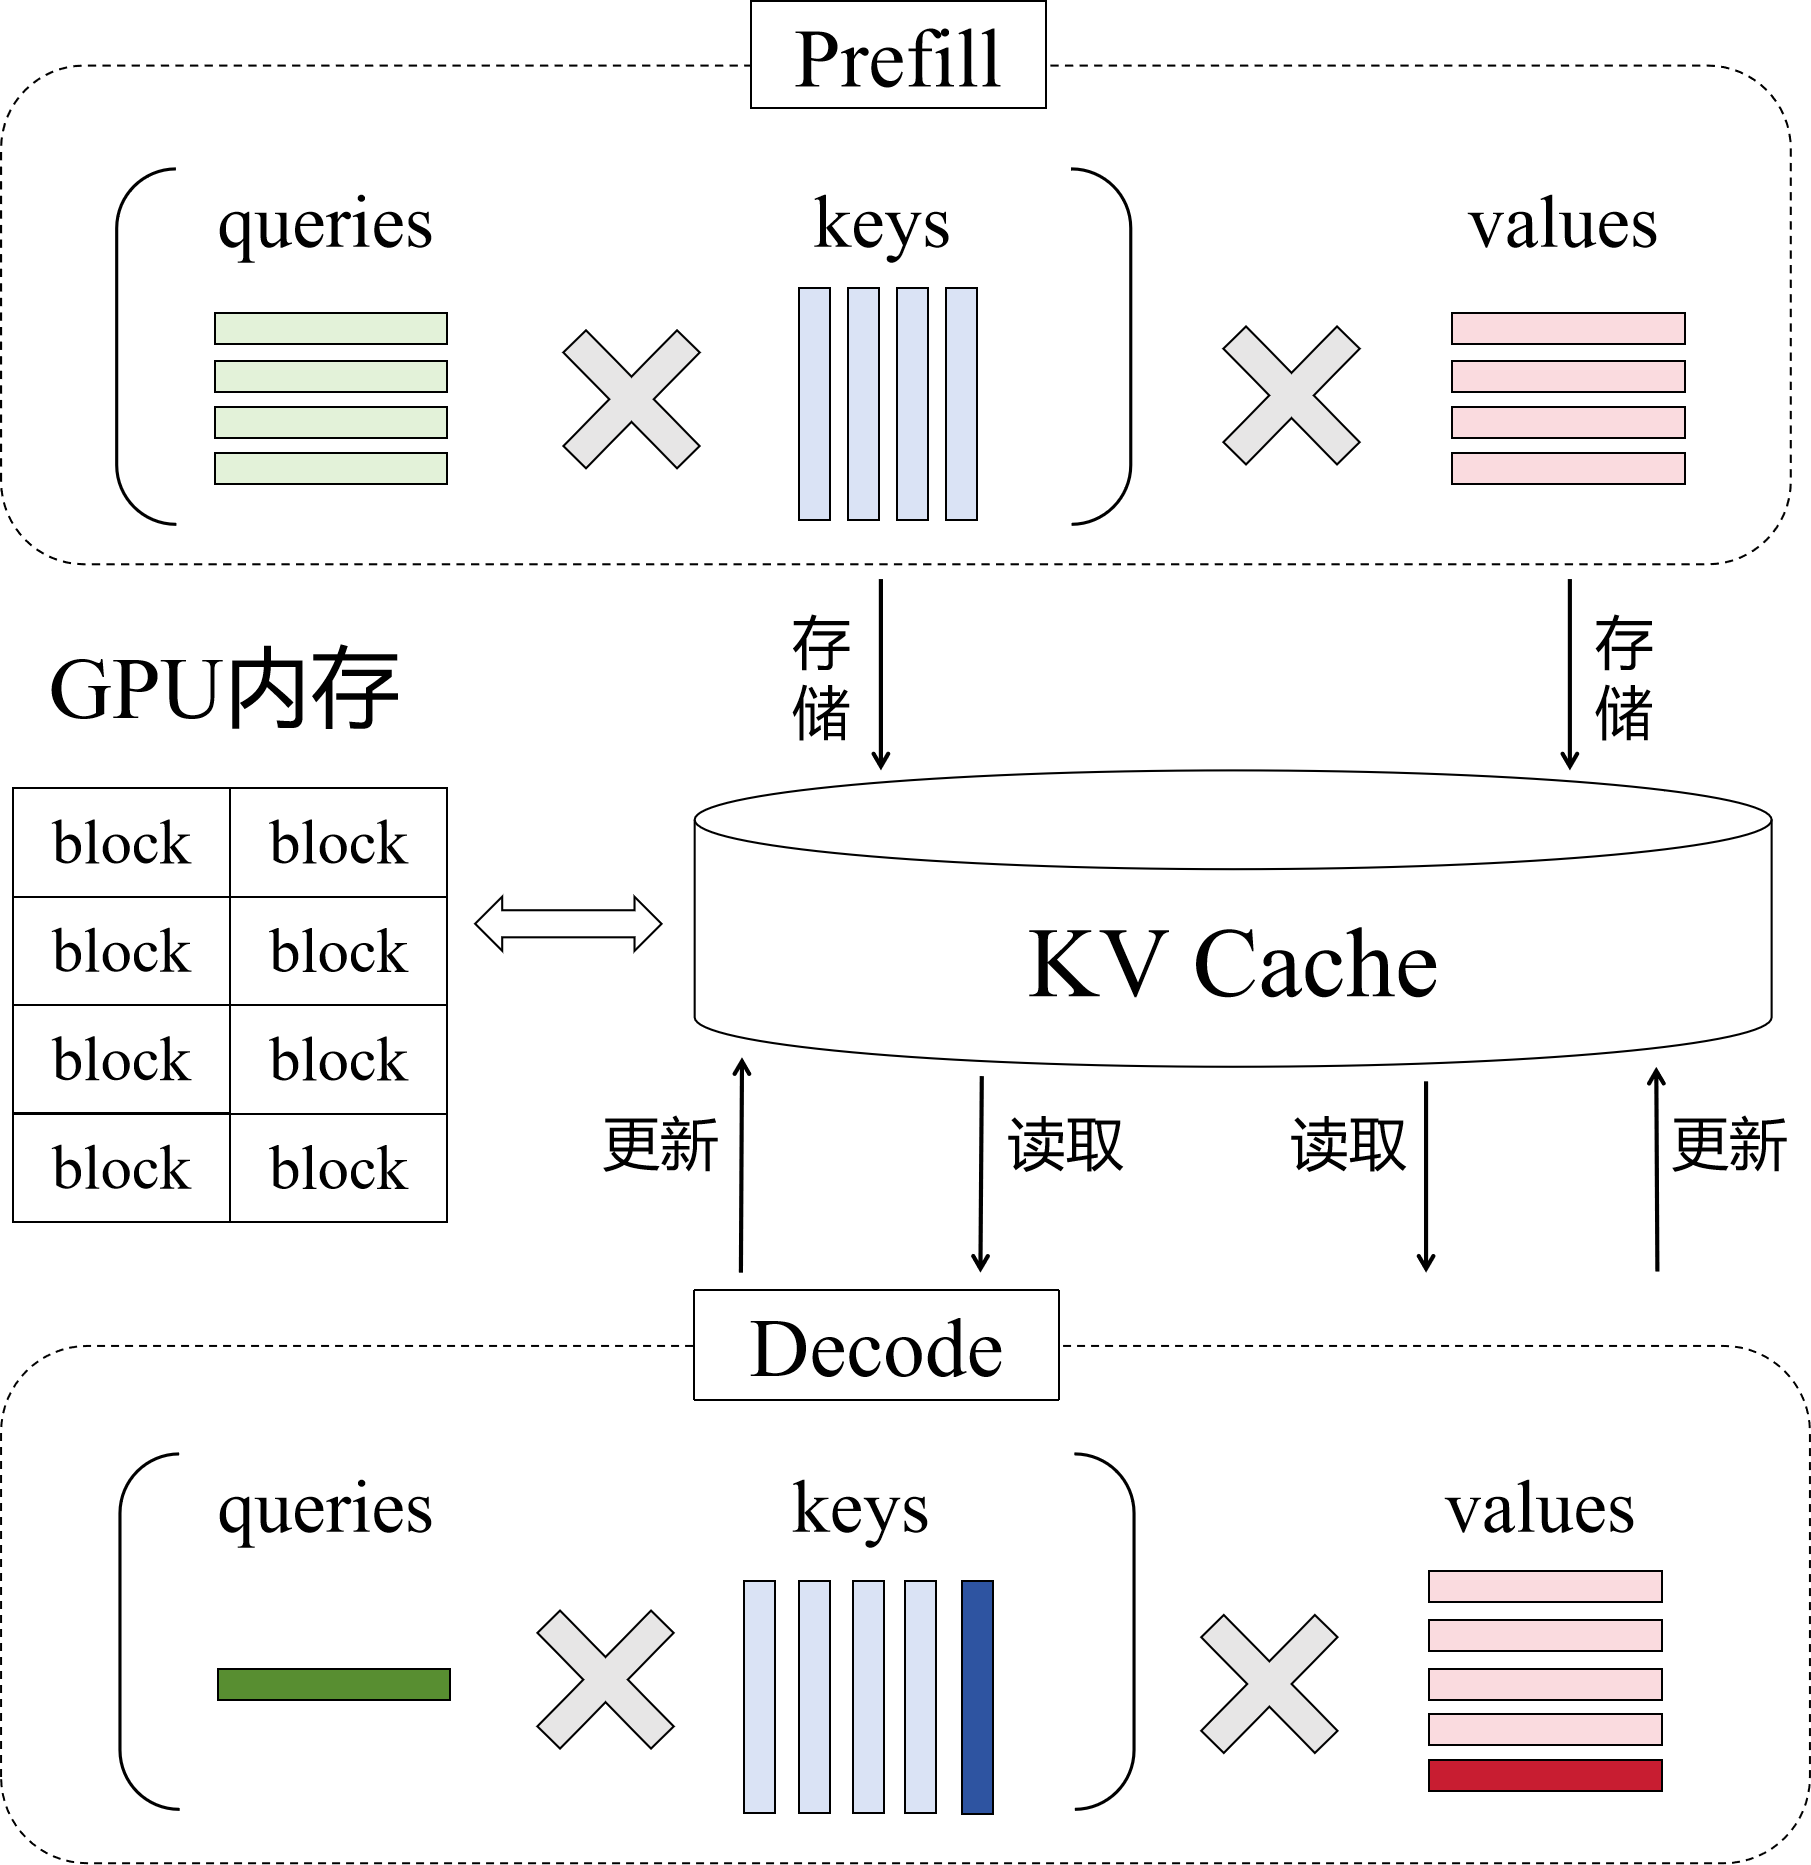
\includegraphics[width=0.9\linewidth]
  {KV Cache的功能示意图.png}
  \caption{KV Cache的功能示意图}
  \label{KV Cache的功能示意图}
\end{figure}

\subsection{KV Cache的优化瓶颈}
KV Cache的引入方便了计算过程,却带来一些挑战,使得LLM推理性能的提升无法达到预期水平,下面列举了三个被人们所广泛讨论和研究的问题。 
\subsubsection{推理内存瓶颈}
随着后续token的不断生成,KV Cache迅速扩展,占用大量GPU内存,产生推理内存瓶颈。在OPT-13B模型中,对于一个长度为100的用户请求,其KV Cache能够占用39.1MB的内存空间。有限的GPU内存将批处理大小限制在较低水平,阻碍推理并发度的进一步提升。
\subsubsection{内存利用率低}
在传统的LLM推理服务框架中,内存管理器按照用户定义的序列长度上限,为每个用户请求设置一块固定大小的GPU内存空间用来存储KV Cache。但由于用户请求长度的差异性,使得GPU内存空间中产生很多内碎片。为了解决内碎片问题,部分LLM推理服务框架能够基于历史信息来预测用户请求的输出长度,并基于预测值来分配内存。然而,预测误差会导致序列的意外截断,且旧请求的完成与新请求的加入使得内存中产生很多外碎片。随着新用户请求的不断到来,内碎片与外碎片在内存中积累,严重影响了内存空间的高效使用。基于这些问题,vLLM框架引入了Paged Attention机制,基于OS中的页式内存管理思想,将GPU内存划分成内存块,并通过维护“KV Cache块表”来支持KV Cache在内存空间中的不连续存储。该机制基本消除了内碎片和外碎片现象,大大提升了内存利用率。 
\subsubsection{通信开销问题}
为了解决推理内存瓶颈问题,人们引入了张量交换技术,将一部分暂时不会使用到的KV Cache保存在CPU中,计算需要时重新传输至GPU中。但此时,有限的PCIe带宽会使得换出和换入过程产生不可忽略的传输通信开销,限制吞吐率,降低推理性能。当张量交换操作所带来的开销已经超过重新调用自注意力机制的开销时,人们选择后一种方式来获取所有前序token的key-value张量,即放弃张量的换出和换入过程,而在用户请求被调度时执行一次prefill操作来代替原本应该执行的decode操作。该过程也被称为张量重算。这些key-value张量在初次生成时经历了多次前向传播操作,而在重算过程中仅仅需要调用自注意力机制过程即可得到,因此张量重算的开销远远小于token序列初次生成时的开销。

\section{相关工作}
本章介绍LLM推理优化领域的国内外研究现状。第一节介绍三种常用的LLM推理优化技术——交换、重算和压缩;第二节列举一些传统的LLM推理框架,并对它们进行优缺点分析。

\subsection{LLM推理张量优化技术}
在LLM推理服务过程中,传统的张量优化技术有三种:张量交换、张量重算和张量压缩(Compression),本文实现了张量交换技术与张量重算技术。而张量压缩技术是下一阶段的工作,目前还未能实现。
\subsubsection{张量交换}
服务器拥有GPU-CPU-磁盘三级存储结构。GPU位于三级存储中的最上层,其计算速率快,并行度高,但存储空间有限,而CPU和磁盘的存储空间相对较大。为了提升服务器的实时吞吐率,LLM推理服务框架一般采用批处理的方式执行用户请求。随着批处理大小的增加或模型参数量的扩展,运行时需要保存的张量会超出GPU的内存限制。当检测到GPU内存占用峰值达到较高水平时,需要开启张量交换功能,将一部分需要保存,而暂时用不到的张量换出到CPU甚至磁盘中,在计算需要时重新换入GPU中。综上所述,张量交换包括换出与换入两个阶段,有两次数据传输过程。
\subsubsection{张量重算}
在抢占式用户请求调度系统中,当某个请求获得执行权时,其会检查之前的计算结果是否保存在GPU中,如果不在,则需要重新获取这部分计算结果。此时可以无需将之前存储的计算结果(如果有)从CPU或磁盘中换入到GPU中,而仅仅对它们进行重新计算。
\subsubsection{张量压缩}
张量压缩技术一般与张量交换技术联合使用。张量交换技术能够有效地利用GPU的计算资源与CPU、磁盘的内存空间,使得大型LLM在有限的GPU内存空间中也能以较大的批处理大小执行推理任务。但是,张量在三级存储结构中的传输会带来无法忽略的通信开销。由于三级存储结构之间的传输带宽是有限的,因此随着LLM参数量和批处理大小的增加,通信开销成为了主要性能瓶颈。压缩技术指通过矩阵变换等数学方式减少参数量。传统工作已经证明,高效的压缩技术能够在不损失张量精度的前提下减小通信开销,进一步提升批处理大小上限,实现更高吞吐率。

\subsection{传统的LLM推理框架}
传统的LLM推理服务框架采取了很多显存优化技术。 \par
Hugging Face Accelerate实现了张量交换技术,但换出与换入的张量仅限于LLM的参数张量;DeepSpeed ZeRO-Inference实现了LLM的分布式推理,能够利用数据并行性与张量并行性来实现LLM推理加速。但以上两个框架均无法针对KV Cache实现交换技术,也没有实现压缩或重算技术。 \par
FlexGen首次提出了“自适应张量优化”的概念,并将张量交换的范围由参数张量扩展至所有张量。通过线性规划建模在交换方案的可行域内进行搜索,在给定的时间内找到较优解。同时,FlexGen还实现了张量压缩技术,相比于Hugging Face Accelerate和DeepSpeed ZeRO-Inference,实现了较大的吞吐率提升。然而,FlexGen假设同一批中的所有用户请求拥有相同的输出长度,在实际情况中,输出长度具有很大的差异性。 \par
为了解决上述问题,ORCA将批处理调度的粒度从单个用户请求转化为单次推理迭代,化解了同一批中用户请求相互等待的性能瓶颈。 \par
vLLM在ORCA的基础上实现了张量重算技术。基于OS中的页式内存管理思想,引入Paged Attention机制来实现。vLLM相比于OCRA,大幅度提升了显存利用率,并增加了批处理大小的上限,进而提升了推理任务的整体吞吐率。本项目将以vLLM作为底层框架进行增量式开发。 \par
另外,其它推理加速技术也被广泛提出和应用。SpecInfer引入了投机推理技术(Speculative Sampling),根据小型LLM的输出来预测大型LLM的输出,在大幅度提升推理吞吐率的同时保障了输出质量。DistillSpec在SpecInfer的基础上实现了知识蒸馏技术(Knowledge Distillation,KD),使得输出预测准确率显著提升。 \par

\section{优化设计}
本章介绍创新工作。第一节给出本文的整体设计方案;第二节介绍张量重算分析器的工作流程;第三节介绍张量交换分析器的工作流程;第四节介绍基于开销感知的张量优化策略;第五节介绍基于公平性的用户请求调度策略。

\subsection{整体架构}
本文的整体设计架构如图\ref{整体设计架构}所示。本文在vLLM框架的基础上进行增量式开发,设计了张量重算分析器、张量交换分析器和自适应LLM推理加速器。 \par
张量重算分析器基于用户请求长度、模型隐藏维度、模型层数等运行时信息来预测重算开销;张量交换分析器基于KV Cache内存占用和GPU-CPU双向传输带宽来预测交换开销。实验环节将会计算二者的预测误差。 \par
自适应LLM推理加速器包含内存优化决策器和用户请求调度器。内存优化决策器引入了基于开销感知的张量优化策略,用于在GPU内存不足时选择开销较小的抢占方式(重算或交换),提升了总体吞吐率,实现了面向服务器端的处理加速;用户请求调度器实现了基于公平性的用户请求调度策略,减少了单请求响应时间,实现了面向客户端的实时处理。 \par

\begin{figure}[!htbp]
  \centering
  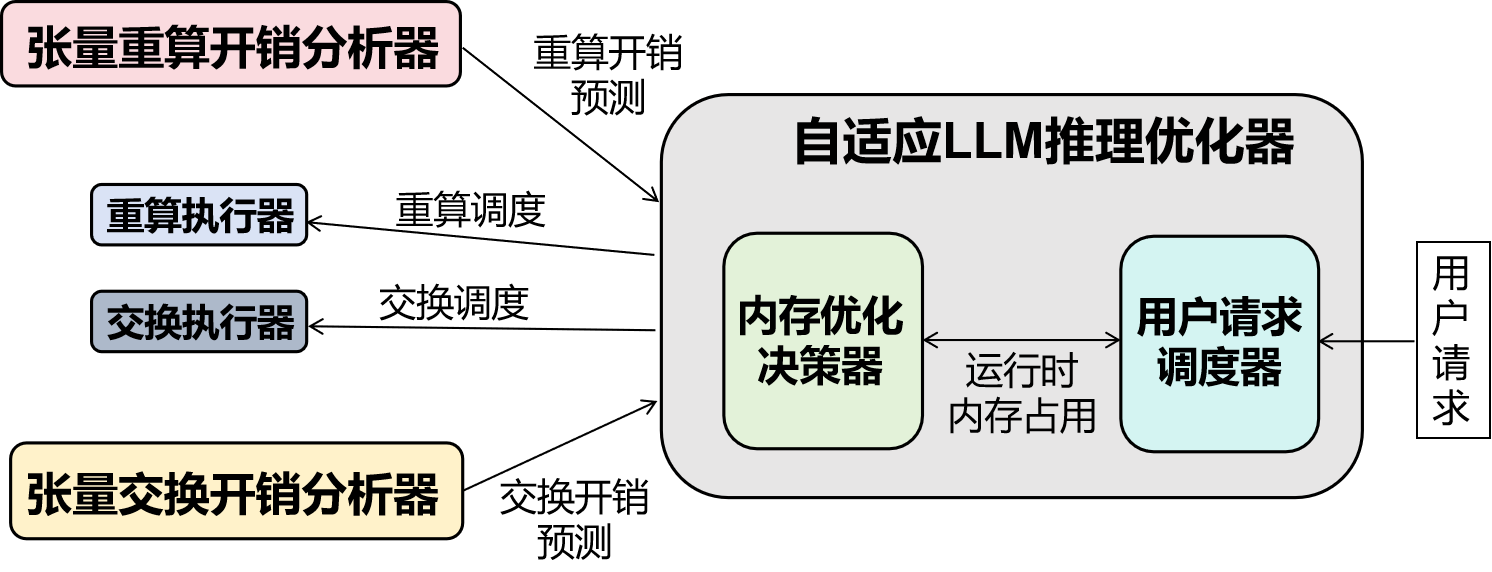
\includegraphics[width=0.9\linewidth]
  {整体设计架构.png}
  \caption{整体设计架构}
  \label{整体设计架构}
\end{figure}
在推理任务执行过程中,内存优化决策器与用户请求调度器共享运行时内存占用信息。在GPU内存不足时,内存优化决策器按照一定的算法选择优先级最低的用户请求进行抢占。其收集张量重算分析器提供的重算开销预测值与张量交换分析器提供的交换开销预测值,选择开销较小的抢占方式,而后交付相应的执行器。用户请求调度器在GPU内存空余时重新调度被抢占的用户请求,在满足公平性的前提下尽可能多地调度用户请求,避免GPU资源的浪费。

\subsection{张量重算分析器}
张量重算的流程如图\ref{张量重算示意图}所示。当用户请求被抢占时,重算执行器在GPU内存中删除其KV Cache;当其被重新调度时,通过一次prefill阶段的执行来恢复被删除的KV Cache数据。因此,张量重算引入的额外开销等于被抢占请求单独执行prefill阶段的时间。本文以OPT和Llama模型为例,通过算子粒度的复杂度分析来找出单步推理时间的影响因素。
\begin{figure}[!htbp]
  \centering
  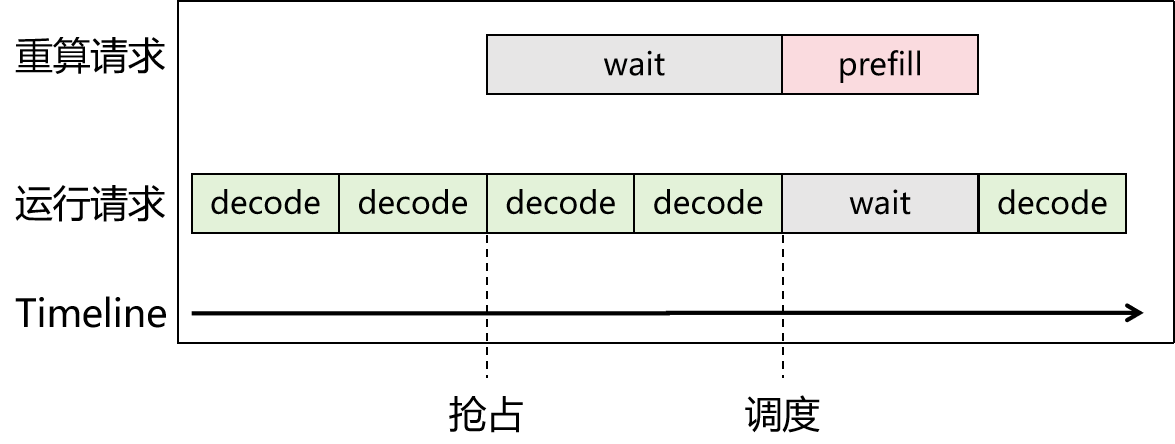
\includegraphics[width=0.9\linewidth]
  {张量重算示意图.png}
  \caption{张量重算示意图}
  \label{张量重算示意图}
\end{figure}

\subsubsection{算子粒度开销分析}
OPT和Llama模型中包含5种不同的算子:ReLU、Norm、Linear、SiluAndMul和Attention,其计算流程如图\ref{四种算子的计算流程}所示。图中$X_i$,$Y_i$是由用户输入决定的张量维度;$input\_dim$,$output\_dim$,$head\_size$是由算子决定的张量维度。 
\par
\begin{figure}[!htbp]
  \centering
  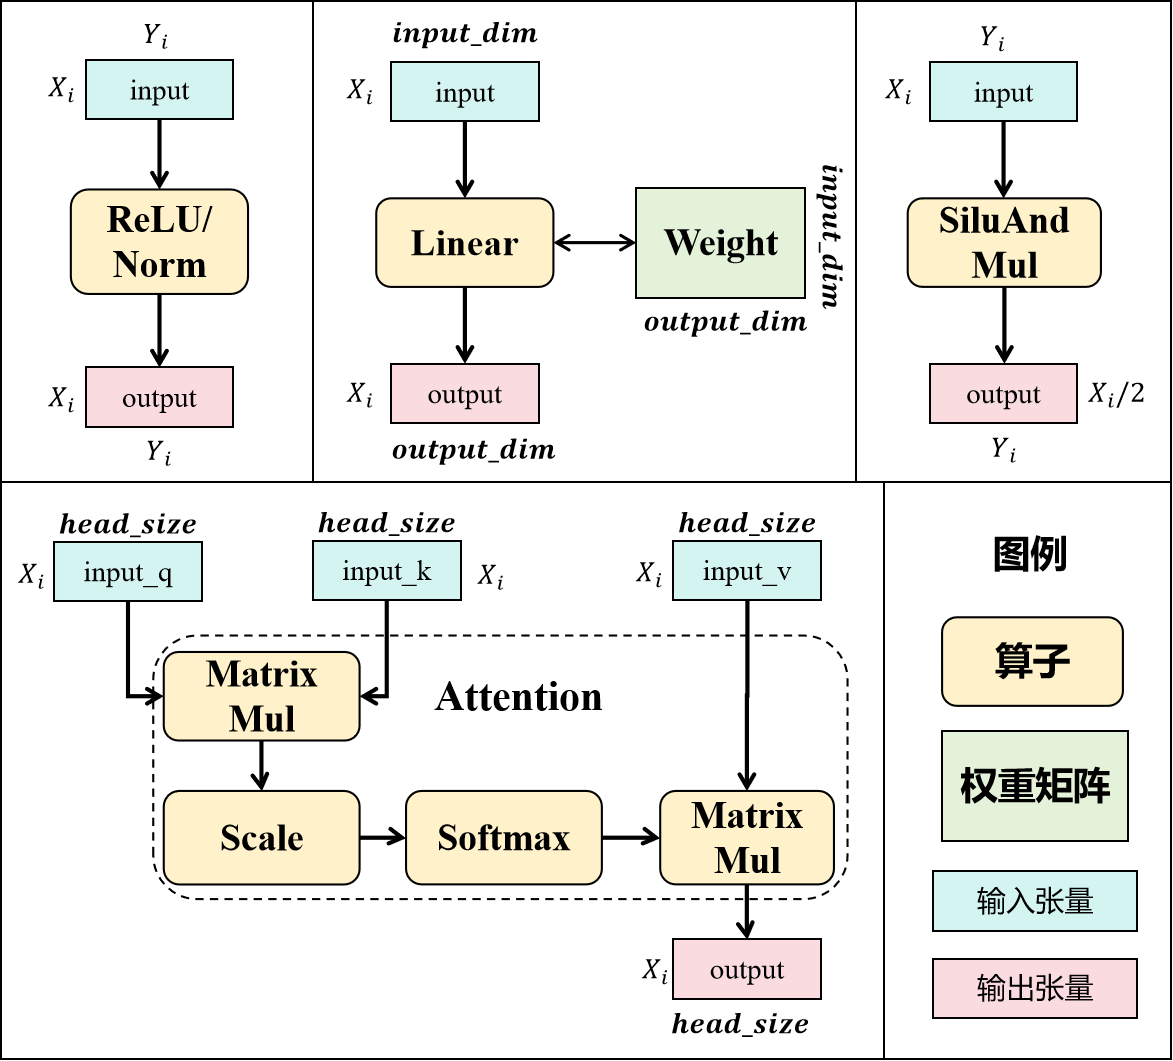
\includegraphics[width=0.9\linewidth]
  {四种算子的计算流程.png}
  \caption{四种算子的计算流程}
  \label{四种算子的计算流程}
\end{figure}

下面分别对这些算子进行复杂度分析。 \par
\begin{itemize}
  \item ReLU算子:逐位调用激活函数进行计算,时间复杂度为$O(X_i*Y_i)$。
  \item Norm算子:是LayerNorm、RMSNorm(仅在Llama模型中)等多种归一化算子的统称,其计算复杂度为$O(X_i*Y_i)$。
  \item Linear算子:是RowParallelLinear,ColumnParallelLinear等多种线性层的统称,将输入向量从$input\_dim$维空间映射到$output\_dim$维空间中,其计算复杂度为$O(X_i*input\_dim*output\_dim)$。
  \item SiluAndMul算子:该算子仅出现在Llama模型的MLP层中,将输入向量的维度减半,其计算复杂度为$O(X_i*Y_i)$。
  \item Attention算子:属于复合操作,由矩阵乘法、缩放和Softmax激活等底层算子组成,整体计算过程如公式\ref{Attention},其计算复杂度为$O(X_i^2*head\_size)$。
  \begin{equation}
    \small
    Attention(Q,K,V)=softmax(\frac{Q\times K^T}{\sqrt{h}}\times V)
    \label{Attention}
  \end{equation}
\end{itemize}
根据算子粒度的复杂度分析,可以找到LLM单步推理执行时间的影响因素,如表\ref{OPT与Llama单次迭代执行时间的影响因素}所示。

\begin{table}[H]
  \centering
  \caption{OPT与Llama单次迭代执行时间的影响因素}
  \label{OPT与Llama单次迭代执行时间的影响因素}
  \begin{tabular}{|c|c|}
    \hline
    \textbf{变量} & \textbf{含义} \\ \hline
    hidden\_size & 模型嵌入维度 \\ \hline
    num\_layers & LLM层数 \\ \hline
    max\_num\_tokens & 单请求需要处理的字符数量 \\ \hline
    batch\_size & 批处理大小 \\ \hline
  \end{tabular}
\end{table}

\subsubsection{单步推理开销预测模型}
单步迭代执行时间预测是一项拥有4个输入变量,1个输出变量的回归预测任务。根据模型层的计算量分析,输出变量与输入变量之间存在多项式依赖关系。因此,本文选用8个回归模型(线性回归模型LR,决策树回归模型DT,随机森林回归模型RF,岭回归模型Ridge,套索回归模型Lasso,弹性回归模型Elastic,梯度提升回归模型GB,K-临近回归模型KNN),并针对每种回归模型,对不同的多项式次数(1到5)进行遍历测试。选择在测试集上预测误差最小者及相应的多项式次数,将其部署到张量重算分析器中。 

\subsection{张量交换分析器}
张量交换的流程如图\ref{张量交换示意图}所示。当用户请求被抢占时,交换执行器将其KV Cache从GPU中传输到CPU中(换出阶段);当该用户请求被重新调度时,将其KV Cache传输回GPU中(换入阶段)。因此,张量交换引入的额外开销等于换出时间与换入时间之和。 \par
\begin{figure}[!htbp]
  \centering
  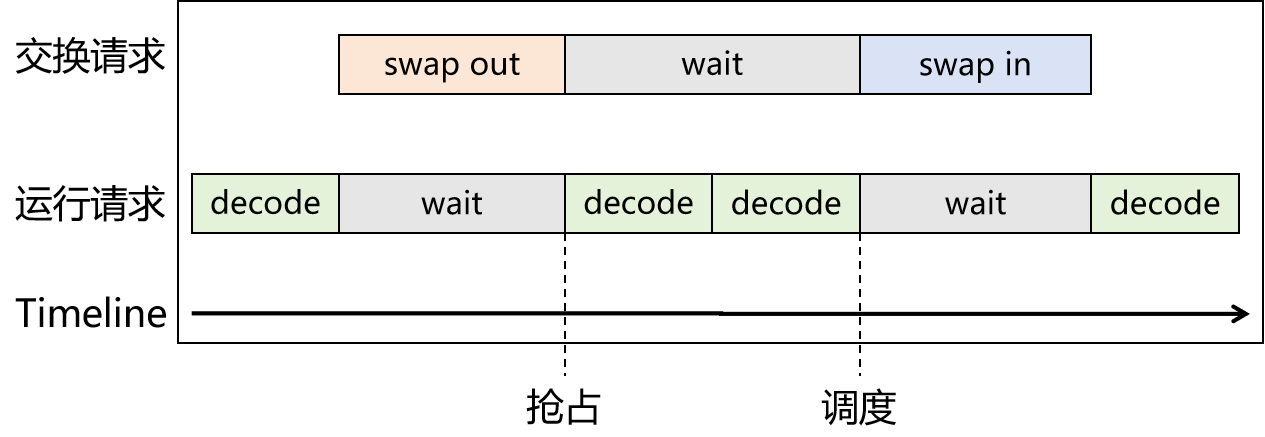
\includegraphics[width=0.9\linewidth]
  {张量交换示意图.png}
  \caption{张量交换示意图}
  \label{张量交换示意图}
\end{figure}

换出开销与换出开销的计算方式如公式\ref{Swap Overhead}所示.
\begin{equation}
  \begin{aligned}
    SwapOut\_Time=\frac{KVCache\_Mem}{DtoH-bandwidth} \\
    SwapIn\_Time=\frac{KVCache\_Mem}{HtoD-bandwidth}
  \end{aligned}
  \label{Swap Overhead}
\end{equation}

vLLM框架采取了PagedAttention技术,将若干token的key-value张量保存在同一个GPU Block中,每个Block占用内存的计算方式为公式\ref{Block Mem},其中是用户定义的参数,用于调整Block大小。
\begin{equation}
  \begin{aligned}
    block\_mem = num\_layers \times hidden\_size \times 
    \\ block\_size \times sizeof(float16)
  \end{aligned}
  \label{Block Mem}
\end{equation}

因此,假设一个用户请求的长度为,其占用GPU block的数量为,则其KV Cache占用的总内存空间为公式\ref{KV Cache Mem}。
\begin{equation}
  \begin{aligned}
    memory = 2 * block\_mem * block\_num =  \\
    2 * block\_mem * \lceil \frac{n}{block\_size} \rceil
  \end{aligned}
  \label{KV Cache Mem}
\end{equation}
由此可以计算出张量交换引入的额外开销。在上述公式中,换入换出传输带宽是由实验环境所决定的,在传输数据量较大时基本保持稳定。是用户定义的参数,由模型参数与用户设置所决定,二者在推理任务中均保持不变。对于不同的用户请求,其区别仅在于序列长度的不同。

\subsection{内存优化决策器}
当GPU内存不足时,需要启动张量优化策略。张量优化策略分为张量交换和张量重算两种。根据上文的分析,张量交换引入的额外开销等于KV Cache的换出开销与换入开销之和;张量重算引入的额外开销等于prefill过程的开销。 \par
张量交换和张量重算所带来的额外开销成为了阻拦用户请求并发度进一步提升的瓶颈,因此抢占方式的选择尤为重要,在不同的运行环境中,应该使用不同的抢占策略来实现较低的抢占开销。然而,vLLM在抢占策略的选择上并未考虑开销问题,针对使用贪心采样策略的用户请求,其使用重算抢占;针对使用并行采样或束搜索采样策略的用户请求,其使用交换抢占。这种固定式抢占策略使得vLLM在面对GPU内存瓶颈时难以有效地压缩开销,进而无法提升吞吐率。本文则对两种抢占方式的开销进行比较,选择开销小的抢占方式执行。内存优化决策器的工作流程如\ref{内存优化决策器工作流程}所示。
\begin{algorithm}
  \caption{Mem\_Schedule}
  \label{内存优化决策器工作流程}
  \begin{spacing}{1.2}
    \begin{algorithmic}[1]
      \REQUIRE {大模型$LLM$, 运行队列$running$, 重算队列$waiting$, 交换队列$swapped$, GPU内存总量$total\_mem$} 
      \ENSURE {无}
      \STATE {$sorted(running, key=priority, order=asc)$}
      \WHILE{$cur\_mem() + LLM.DECODE(running)\newline > total\_mem$}
        \STATE {$req\gets running.pop()$}
        \STATE {$recomp\_time\gets GET\_RECOMP\_TIME()$}
        \STATE {$swap\_time\gets GET\_SWAP\_TIME()$}
        \IF {$swap\_time < recomp\_time$}
          \STATE {$SWAP(req)$} \hfill {// 交付张量交换执行器}
          \STATE {$swapped.append(req)$}
        \ELSE
          \STATE {$RECOMP(req)$} \hfill {// 交付张量重算执行器}
          \STATE {$waiting.append(req)$}
        \ENDIF
      \ENDWHILE
      \RETURN $L'$
    \end{algorithmic}
  \end{spacing}
\end{algorithm}
当剩余的GPU内存空间不足以存放当前用户请求批次在下一个迭代后产生的KV Cache时(第2行),内存优化决策器进入工作状态。其选择当前批次中优先级最低的用户请求(第3行),调用张量交换分析器和张量重算分析器来预测其交换和重算开销(第4、5行)。如果交换开销小于重算开销,则将该请求交付交换执行器处理(第7、8行);否则交付重算执行器处理(第10、11行)。以上过程循环执行,直至当前批次在下一个迭代中产生的KV Cache能够全部存放到GPU内存中。

\subsection{用户请求调度器}
本文维护三个用户请求队列:waiting队列、running队列与swapped队列。waiting队列存储初次进入调度系统,还未执行过,或者因张量重算而失去KV Cache的用户请求;running队列存储正在运行(执行decode阶段)的用户请求;swapped队列存储被换出到CPU中的用户请求。这三个队列之间拥有以下调度规则: \par
\begin{itemize}
  \item running队列中的用户请求运行完毕后会返回客户端,否则继续运行。
  \item 当GPU内存条件允许时,swapped队列中的用户请求可以直接转移至running队列中。
  \item 当GPU内存条件允许时,waiting队列中的用户请求可以转移至running队列中,但需要先执行prefill阶段。
\end{itemize}
如果剩余的GPU空间不足以存储running队列在下一次迭代中产生的KV Cache,则需要内存优化决策器进行抢占调度;如果剩余的GPU空间足够,则考虑扩充running队列,以避免浪费GPU资源。在扩充running队列时,用户请求调度器将部分请求从swapped队列或waiting队列中转移至running队列中。但由于两种转移方式存在较大差别(是否需要执行prefill阶段),因此每次扩充running队列时,或者仅从swapped队列进行调度,或者仅从waiting队列进行调度,而无法同时调度两个队列。用户请求调度器的工作流程如\ref{用户请求调度器工作流程}所示。

\begin{algorithm}
  \caption{Req\_Schedule}
  \label{用户请求调度器工作流程}
  \begin{spacing}{1.15}
    \begin{algorithmic}[1]
      \REQUIRE {待执行的用户请求队列$L$}, {大模型$LLM$}, \newline {GPU内存总量$total$} 
      \ENSURE {用户请求完成状态$Status$}
      \STATE {$w\gets L$}  \hfill {// 初始化waiting队列}
      \STATE {$r\gets empty\_list$} \hfill {// 初始化running队列}
      \STATE {$s\gets empty\_list$} \hfill {// 初始化swapped队列}
      \WHILE {$\neg w.is\_empty()\lor \neg s.is\_empty() \newline \lor \neg r.is\_empty()$}
        \STATE {$MemSchedule(LLM, r, w, s, total, cur)$}
        \STATE {$sorted(s, key=priority, order=asc)$}
        \STATE {$sorted(r, key=priority, order=asc)$}
        \STATE {$s\_sche\gets s$} \hfill {// 从swapped队列调度}
        \WHILE {$cur() + PREFILL\_MEM(s\_sche)\newline >total$}
          \STATE {$s\_sche.pop()$}  
        \ENDWHILE
        \STATE {$w\_sche\gets w$} \hfill {// 从waiting队列调度}
        \WHILE {$cur() + DECODE\_MEM(w\_sche) +\newline DECODE\_MEM(r) > total$}
          \STATE {$w\_sche.pop()$}
        \ENDWHILE
        \STATE {$w\_sche\_pri=GET\_PRIORITY(w\_sche)$}
        \STATE {$s\_sche\_pri=GET\_PRIORITY(s\_sche)$}
        \IF {$w\_sche\_pri\leq s\_sche\_pri$}
          \FOR {$req$ \textbf{in} $s\_sche$}
            \STATE {$r.append(req)$}
            \STATE {$s.remove(req)$}
          \ENDFOR
        \ELSE
          \STATE {$LLM.PREFILL(w\_sche)$}
          \FOR {$req$ \textbf{in} $w\_sche$}
            \STATE {$r.append(req)$}
            \STATE {$w.remove(req)$}
          \ENDFOR
          \STATE \textbf{continue}
        \ENDIF
        \IF {$r.is\_empty()$}
          \RETURN \FALSE \hfill {// running队列为空,无法执行}
        \ELSE
          \STATE {$LLM.DECODE(r)$} \hfill {// 单次推理迭代}
          \FOR {$req$ \textbf{in} $r$}
            \IF {$req.is\_finished()$}
              \STATE {$r.remove(r)$} \hfill {// 移除完成的请求}
            \ENDIF
          \ENDFOR
        \ENDIF
      \ENDWHILE
      \RETURN \TRUE \hfill {// 所有请求均执行完毕}
    \end{algorithmic}
  \end{spacing}
\end{algorithm}

客户端发送的用户请求进入$waiting$队列中,而$running$队列和$swapped$队列最初为空(第1-3行)。当GPU内存不足时,调用内存优化算法进行抢占调度(第5行),否则扩充$running$队列。 \par
用户请求调度器尽可能多地寻找能从$swapped$队列转移至$running$队列的用户请求(第8-11行),和能从$waiting$队列转移至$running$队列的用户请求(第12-15行)。对它们进行优先级比较(第16-17行),若前者的优先级均值较高,则将其直接转移到$running$队列中(第18-22行);若后者的优先级均值较高,则其执行prefill阶段后(第24行)转移至$running$队列中(第25-28行),同时直接进入下一轮迭代(第29行)。需要注意的是,当GPU内存不足时,无法实现从$swapped$队列或$waiting$队列向$running$队列的调度,即$w\_sche$和$s\_sche$队列均为空,此时也就不存在后续的优先级比较过程了。 \par
在以上调度操作完成后,$running$队列应当为非空的,否则推理过程无法继续(第31-32行)。$running$队列执行decode阶段(第34行),将已完成的用户请求移除后进入下一次迭代(第35到39行)。 \par
对于一个用户请求,定义其优先级等于处理时间除以序列长度。处理时间等于当前时刻减去该用户请求初次进入waiting队列的时刻,而序列长度指用户输入与已生成tokens的总长度。定义用户请求队列的优先级等于所有用户请求优先级的平均值。当用户请求初次进入waiting队列时,其序列长度较短,因此优先级增长较为迅速,能够被很快处理;而在用户请求等待过程中,其优先级在不断提升,因此避免了饥饿现象。 \par
vLLM基于FCFS策略进行设计,在调度时优先考虑swapped队列,只有当swapped队列为空时才调度waiting队列,使得以交换方式被抢占的用户请求相比于以重算方式被抢占的用户请求,其重调度的优先级更高。结合上一小节关于vLLM固定式抢占策略的分析可知,一部分用户请求被抢占后能够很快重新调度,而也有一部分用户请求被抢占后进入waiting队列的末位,需要长时间等待。这种调度策略违反了公平性原则。本文中的用户请求调度器基于公平性原则而设计,同时在实验部分证明,其能够大幅提升用户请求的实时性。

\section{实验验证}
本章介绍实验部分。第一节介绍实验平台的软硬件配置;第二节介绍LLM与数据集的选取,以及实验组的设置;第三节分析单步迭代执行时间预测误差;第四节针对基于开销感知的张量优化策略,进行吞吐率优化测试;第五节针对基于公平性的用户请求调度策略,进行实时性测试;第六节进行了一些其它测试工作。

\subsection{实验环境}
本文开展实验使用的服务器软硬件配置如表\ref{实验平台的软硬件配置}所示。使用Intel(R) Xeon(R) CPU和NVIDIA A800 80GB GPU,CUDA版本为11.8。使用pytorch 2.0.l和vllm 0.2.5作为底层框架进行开发。
\begin{table}[H]
  \centering
  \caption{实验平台的软硬件配置}
  \label{实验平台的软硬件配置}
  \begin{tabular}{|c|c|}
    \hline
    \textbf{软件/硬件} & \textbf{型号/版本} \\ \hline
    CPU & Intel(R) Xeon(R) CPU @ 2.60GHz  \\ \hline
    GPU & NVIDIA A800 PCIE 80GB \\ \hline
    OS & CentOS Linux 7 (Core) \\ \hline
    CUDA & 11.8 \\ \hline
    pytorch & 2.0.1 \\ \hline
    vllm & 0.2.5 \\ \hline
  \end{tabular}
\end{table}
服务器使用PCIe实现GPU-CPU通信,PCIe双向传输带宽如表\ref{PCIe双向传输带宽}所示。PCIe传输带宽在不同数据大小下差异显著,在计算张量交换开销时,需要根据单次实际传输的数据量找到对应的传输带宽值。
\begin{table}[H]
  \centering
  \caption{PCIe双向传输带宽}
  \label{PCIe双向传输带宽}
  \begin{tabular}{|c|c|c|}
    \hline
    \textbf{传输量(B)} & \textbf{HtoD(MB/s)} & \textbf{DtoH(MB/s)} \\ \hline
    1024 & 0.19 & 0.24 \\ \hline
    2048 & 0.60 & 0.72 \\ \hline
    4096 & 1.20 & 1.49 \\ \hline
    8192 & 1.07 & 2.97 \\ \hline
    16384 & 4.16 & 5.79 \\ \hline
    32768 & 7.76 & 9.35 \\ \hline
    102400 & 14.27 & 16.49 \\ \hline
    204800 & 18.30 & 20.24 \\ \hline
    409600 & 21.17 & 22.57 \\ \hline
    819200 & 22.63 & 24.04 \\ \hline
  \end{tabular}
\end{table}

\subsection{实验设置}
本文选用OPT和Llama作为实验模型,在三个常见数据集上进行测试,如表\ref{实验数据集选取}所示。图\ref{序列长度分布曲线}绘制了数据集输入长度的分布律曲线。
\begin{table}[H]
  \centering
  \caption{实验数据集选取}
  \label{实验数据集选取}
  \begin{tabular}{|c|c|c|} \hline
    \textbf{数据集} & \textbf{样本总数} & \textbf{平均输入长度} \\ \hline
    Writing & 258042 & 20.0 \\ \hline
    Chatbot & 673 & 17.0 \\ \hline
    Alpaca & 68912 & 19.7 \\ \hline
  \end{tabular}
\end{table}

\begin{figure}[!htbp]
  \centering
  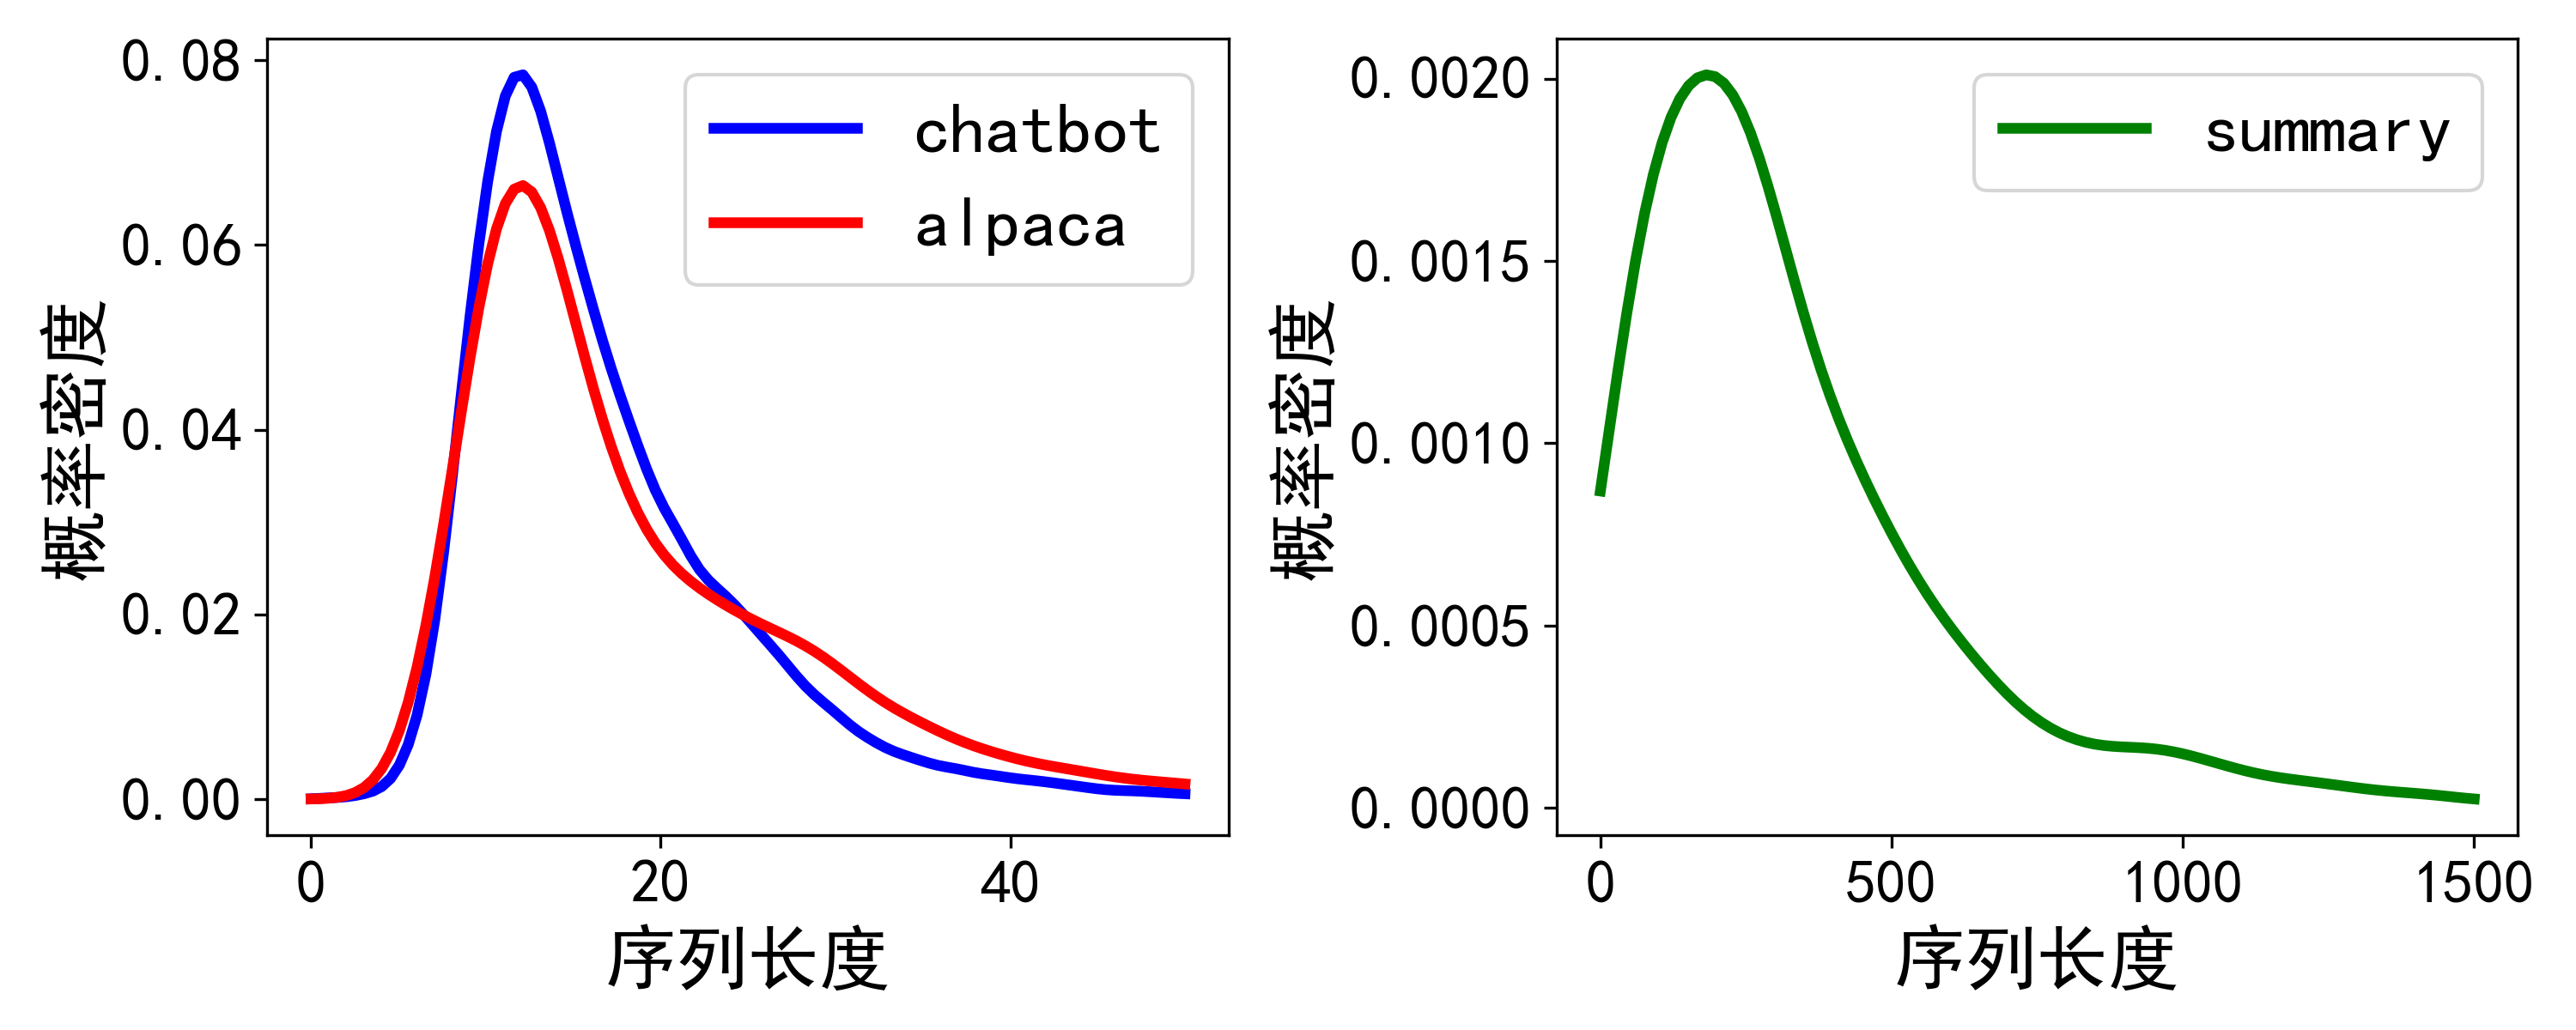
\includegraphics[width=0.9\linewidth]
  {序列长度分布曲线.png}
  \caption{序列长度分布曲线}
  \label{序列长度分布曲线}
\end{figure}

本文共设置了12个实验组,每组在相应数据集中随机选取一部分作为测试数据,详细信息见表5.实验组设置过程中遵循以下原则:
\begin{itemize}
  \item 将GPU内存利用率设置在较低水平,使得推理任务只有在频繁执行抢占操作时才能正常执行。
  \item 在输出样例数量和最大输出长度的设置上,尽量保证推理任务的总用时在2min到3min之间,方便后续作图。
\end{itemize}

\begin{table}[H]
  \centering
  \caption{实验组设置}
  \label{实验组设置}
  \begin{tabular}{|c|c|c|c|} \hline
    \textbf{实验组编号} & \textbf{1} & \textbf{2} & \textbf{3} \\ \hline
    \textbf{模型} & \multicolumn{3}{|c|}{OPT} \\ \hline
    $hidden\_size$ & \multicolumn{3}{|c|}{3072} \\ \hline
    $num\_layers$ & \multicolumn{3}{|c|}{256} \\ \hline
    GPU利用率 & \multicolumn{3}{|c|}{0.38} \\ \hline
    数据集 & Writing & Chatbot & Alpaca \\ \hline
    测试样例数量 & 100 & 100 & 100 \\ \hline
    最大输出长度 & 128 & 128 & 128 \\ \hline
    \textbf{实验组编号} & \textbf{4} & \textbf{5} & \textbf{6} \\ \hline
    模型 & \multicolumn{3}{|c|}{OPT} \\ \hline
    $hidden\_size$ & \multicolumn{3}{|c|}{4096} \\ \hline
    $num\_layers$ & \multicolumn{3}{|c|}{128} \\ \hline
    GPU利用率 & \multicolumn{3}{|c|}{0.31} \\ \hline
    数据集 & Writing & Chatbot & Alpaca \\ \hline
    测试样例数量 & 180 & 180 & 150 \\ \hline
    最大输出长度 & 160 & 144 & 160 \\ \hline
    \textbf{实验组编号} & \textbf{7} & \textbf{8} & \textbf{9} \\ \hline
    模型 & \multicolumn{3}{|c|}{Llama} \\ \hline
    $hidden\_size$ & \multicolumn{3}{|c|}{3072} \\ \hline
    $num\_layers$ & \multicolumn{3}{|c|}{256} \\ \hline
    GPU利用率 & \multicolumn{3}{|c|}{0.45} \\ \hline
    数据集 & Writing & Chatbot & Alpaca \\ \hline
    测试样例数量 & 100 & 120 & 100 \\ \hline
    最大输出长度 & 160 & 144 & 144 \\ \hline
    \textbf{实验组编号} & \textbf{10} & \textbf{11} & \textbf{12} \\ \hline
    模型 & \multicolumn{3}{|c|}{Llama} \\ \hline
    $hidden\_size$ & \multicolumn{3}{|c|}{4096} \\ \hline
    $num\_layers$ & \multicolumn{3}{|c|}{128} \\ \hline
    GPU利用率 & \multicolumn{3}{|c|}{0.35} \\ \hline
    数据集 & Writing & Chatbot & Alpaca \\ \hline
    测试样例数量 & 160 & 150 & 150 \\ \hline
    最大输出长度 & 160 & 160 & 160 \\ \hline
  \end{tabular}
\end{table}

\subsection{执行时间预测}
表\ref{OPT模型单步迭代执行时间预测误差}和表\ref{LLama模型单步迭代执行时间预测误差}分别展示了OPT模型和Llama模型单步推理执行时间的预测效果。在OPT执行时间预测任务中,随机森林回归模型性能最佳,其在拟合2次多项式时能够达到1.76\%的预测误差;在Llama执行时间预测任务中,随机森林模型同样性能最佳,其在拟合2次多项式时能够达到1.30\%的预测误差。

\begin{table}[H]
  \centering
  \caption{OPT模型单步迭代执行时间预测误差}
  \label{OPT模型单步迭代执行时间预测误差}
  \small
  \begin{tabular}{|c|c|c|c|c|c|}
    \hline
    \textbf{模型-拟合次数} & \textbf{1} & \textbf{2} & \textbf{3} & \textbf{4} & \textbf{5} \\ \hline
    线性回归模型 & 76.41 & 69.44 & 39.61 & 12.91 & 9.18 \\ \hline
    决策树 & 1.30 & 1.31 & 1.31 & 1.31 & 1.30 \\ \hline
    随机森林 & 1.33 & 1.32 & 1.34 & 1.34 & 1.34 \\ \hline
    岭回归模型 & 76.41 & 69.01 & 39.18 & 12.73 & 7.72 \\ \hline
    lasso回归模型 & 69.23 & 33.57 & 34.42 & 35.16 & 31.58  \\ \hline
    弹性回归模型 & 127.18 & 139.7 & 100.18 & 94.94 & 93.51  \\ \hline
    梯度提升模型 & 22.42 & 21.97 & 19.42 & 19.99 & 19.38  \\ \hline
    KNN回归模型 & 2.24 & 2.36 & 2.48 & 2.63 & 2.68 \\ \hline
  \end{tabular}
\end{table}

\begin{table}[H]
  \centering
  \caption{LLama模型单步迭代执行时间预测误差}
  \label{LLama模型单步迭代执行时间预测误差}
  \small
  \begin{tabular}{|c|c|c|c|c|c|}
    \hline
    \textbf{模型-拟合次数} & \textbf{1} & \textbf{2} & \textbf{3} & \textbf{4} & \textbf{5} \\ \hline
    线性回归模型 & 46.52 & 46.65 & 28.75 & 11.86 & 9.32 \\ \hline
    决策树 & 1.81 & 1.81 & 1.81 & 1.81 & 1.81 \\ \hline
    随机森林 & 1.77 & 1.76 & 1.77 & 1.77 & 1.78 \\ \hline
    岭回归模型 & 46.52 & 46.37 & 28.45 & 11.51 & 7.36 \\ \hline
    lasso回归模型 & 40.22 & 25.53 & 27.38 & 26.08 & 25.49 \\ \hline
    弹性回归模型 & 111.89 & 123.62 & 91.67 & 87.59 & 86.48 \\ \hline
    梯度提升模型 & 15.57 & 16.05 & 14.80 & 15.09 & 14.68 \\ \hline
    KNN回归模型 & 2.55 & 2.80 & 2.89 & 3.00 & 3.05 \\ \hline
  \end{tabular}
\end{table}

\subsection{吞吐率测试}
张量重算开销随着序列长度的增加而缓慢增加。究其根本,prefill阶段的开销之所以大于相同条件下decode阶段的开销,是因为单次迭代处理字符数量的增加导致自注意力层的总计算量增加。自注意力机制内核采用了并行计算策略,每个线程只计算一个字符的qkv张量及注意力值。输入字符增加使得并行执行的线程数量增加,而非每个线程的计算量,因此增加的只是线程间的同步开销。而由公式\ref{Swap Overhead}、\ref{Block Mem}、\ref{KV Cache Mem}可知,张量交换开销与序列长度成近似正比关系。因此,张量重算开销的增长速度小于张量交换开销。 \par
本文对实验组1和实验组7进行开销对比测试,其结果如图\ref{交换与重算开销对比}所示。当序列长度较小时,交换开销小于重算开销;随着序列长度的增加,交换开销等比增加,而重算开销增加缓慢,使得二者的大小关系反转。 \par
因此,对于长序列,无论是vLLM策略还是本文策略,都偏向于使用重算,两种策略所带来的抢占行为没有差异。对于短序列,vLLM策略使用重算,而本文策略使用开销较小的交换,此时能够带来吞吐率提升。在LLM实际应用场景中,大多数序列的长度较短,使得张量交换在提升性能上拥有明显优势。 \par
\begin{figure}[!htbp]
  \centering
  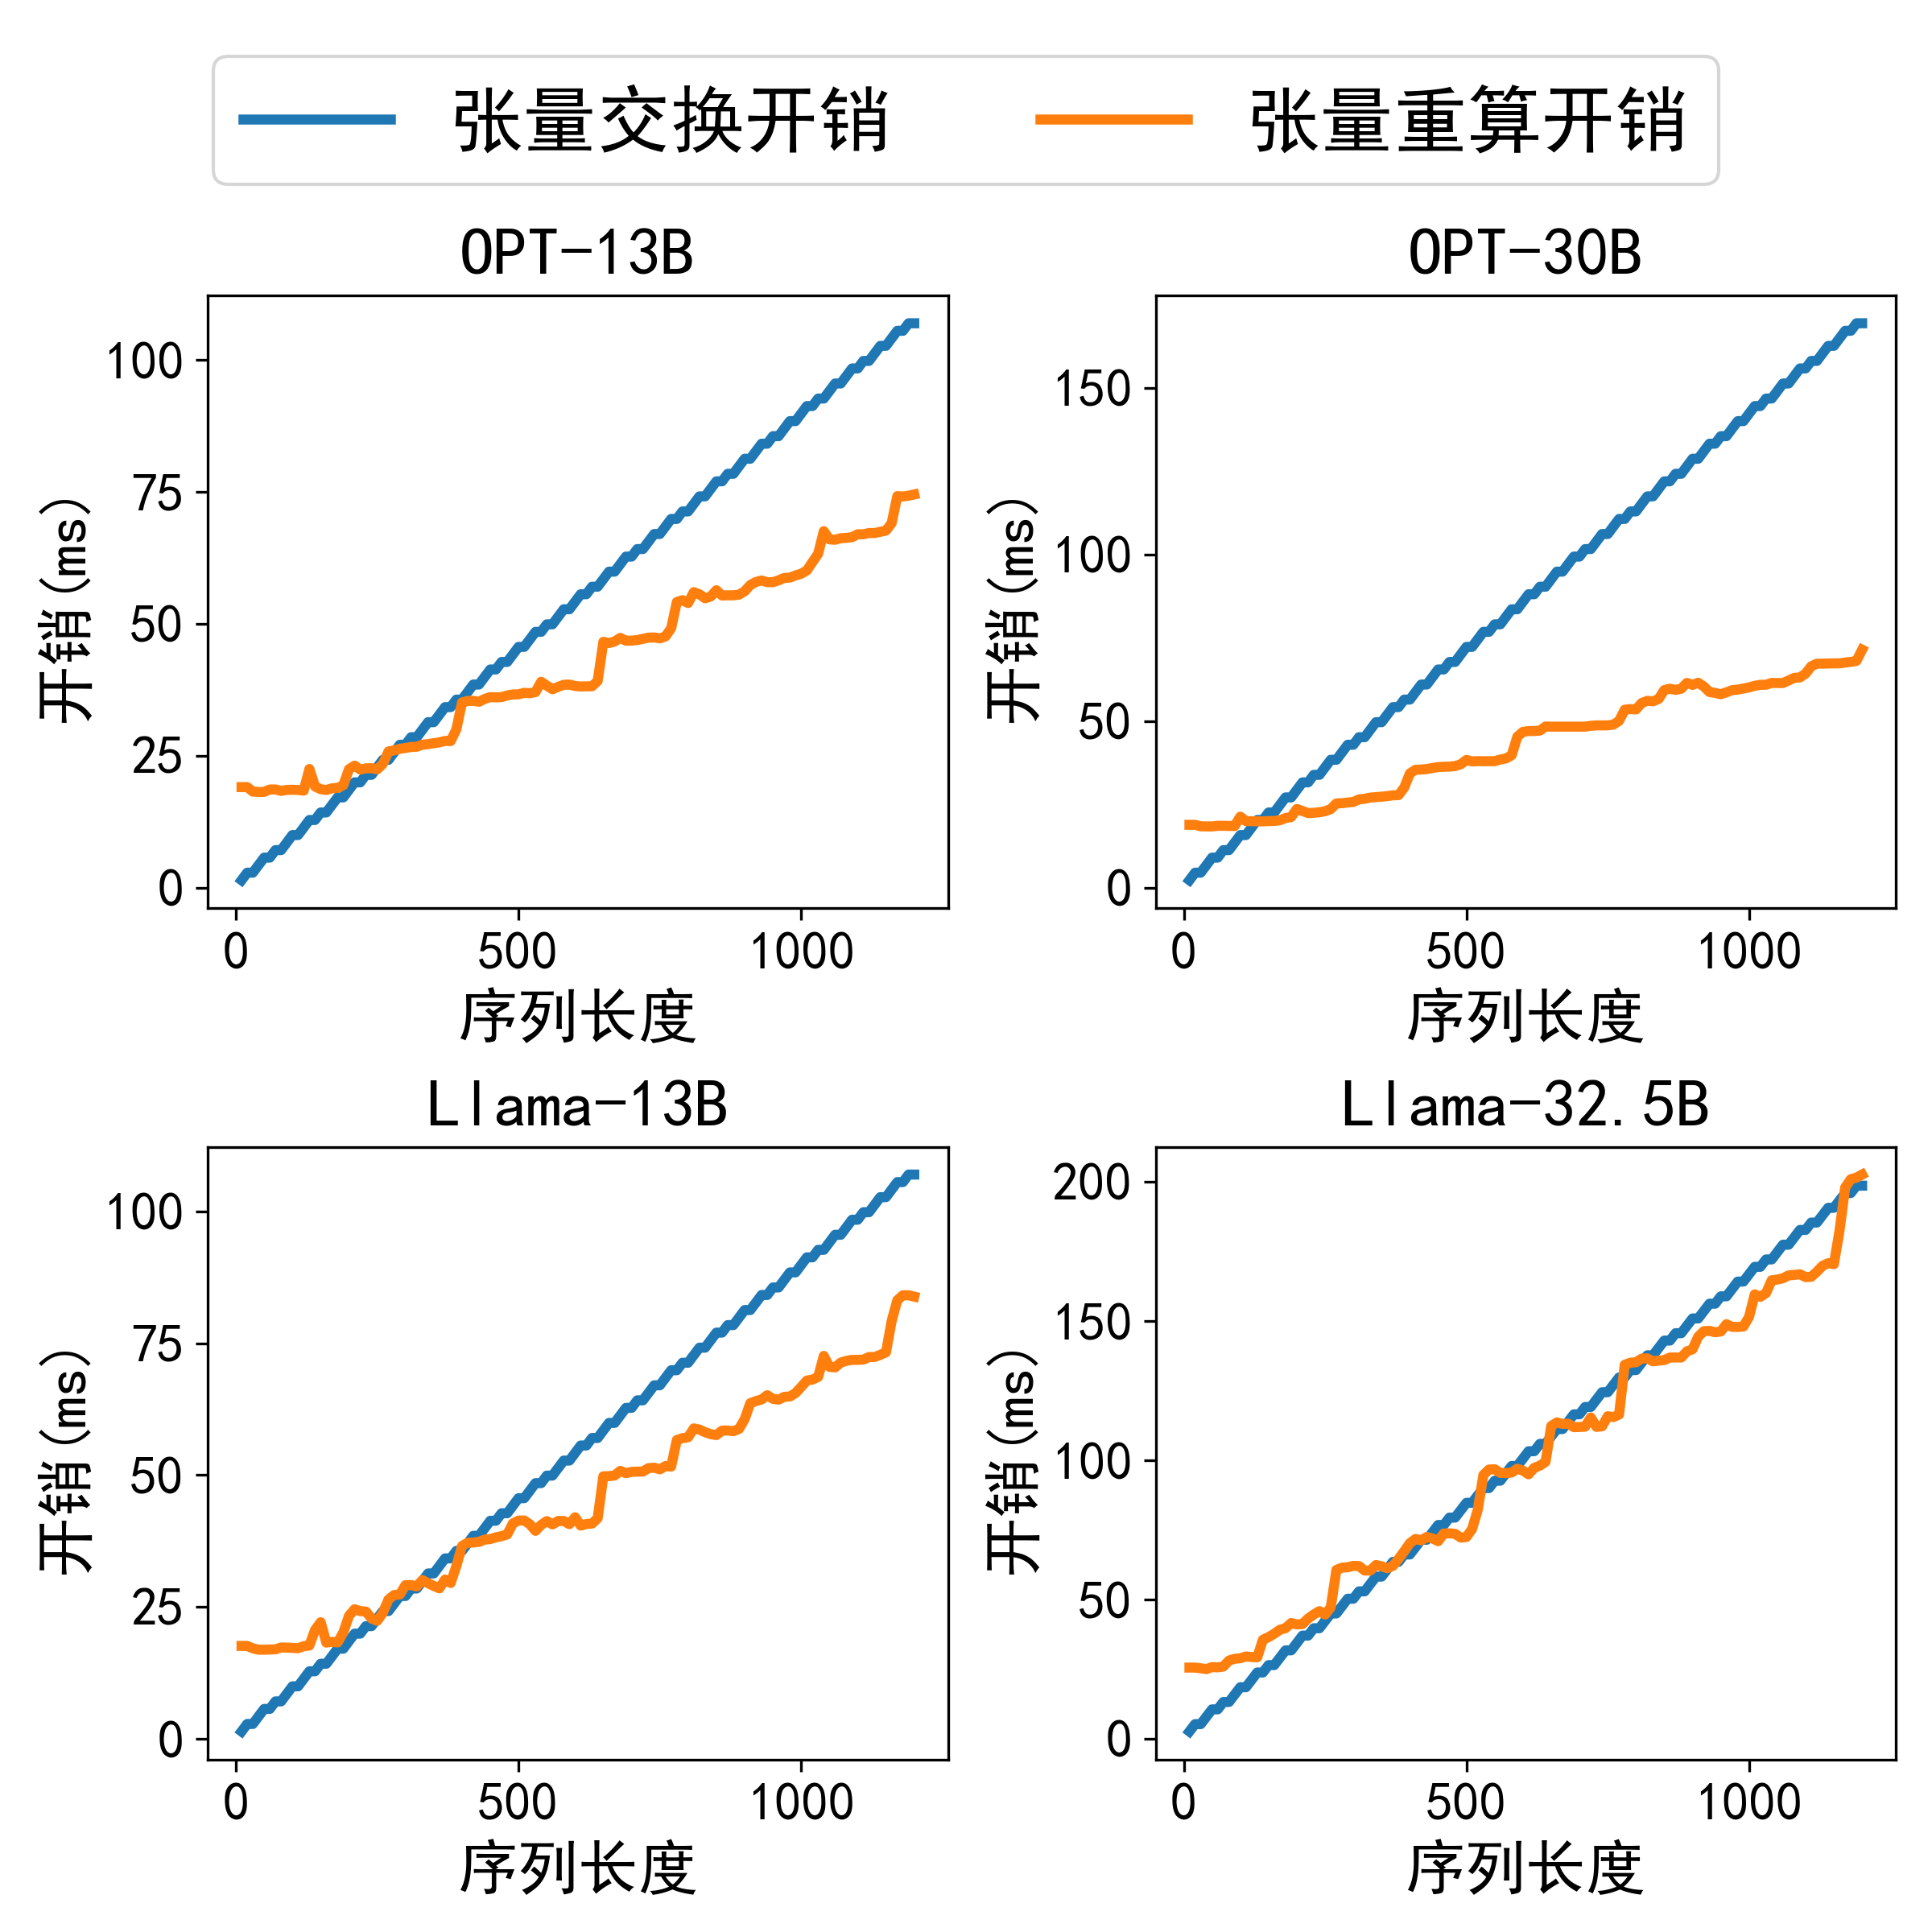
\includegraphics[width=0.9\linewidth]
  {交换与重算开销对比.png}
  \caption{交换与重算开销对比}
  \label{交换与重算开销对比}
\end{figure}
图\ref{推理任务总用时}展示了12个实验组推理任务的总用时,表\ref{本文策略在12个实验组中的加速比}给出了本文策略相比于vLLM策略在12个实验组中的加速比。图ref{用户请求抢占次数}记录了推理过程中的抢占行为。结果表明,本文策略能够实现1.2到1.4的整体加速比。
\begin{figure}[!htbp]
  \centering
  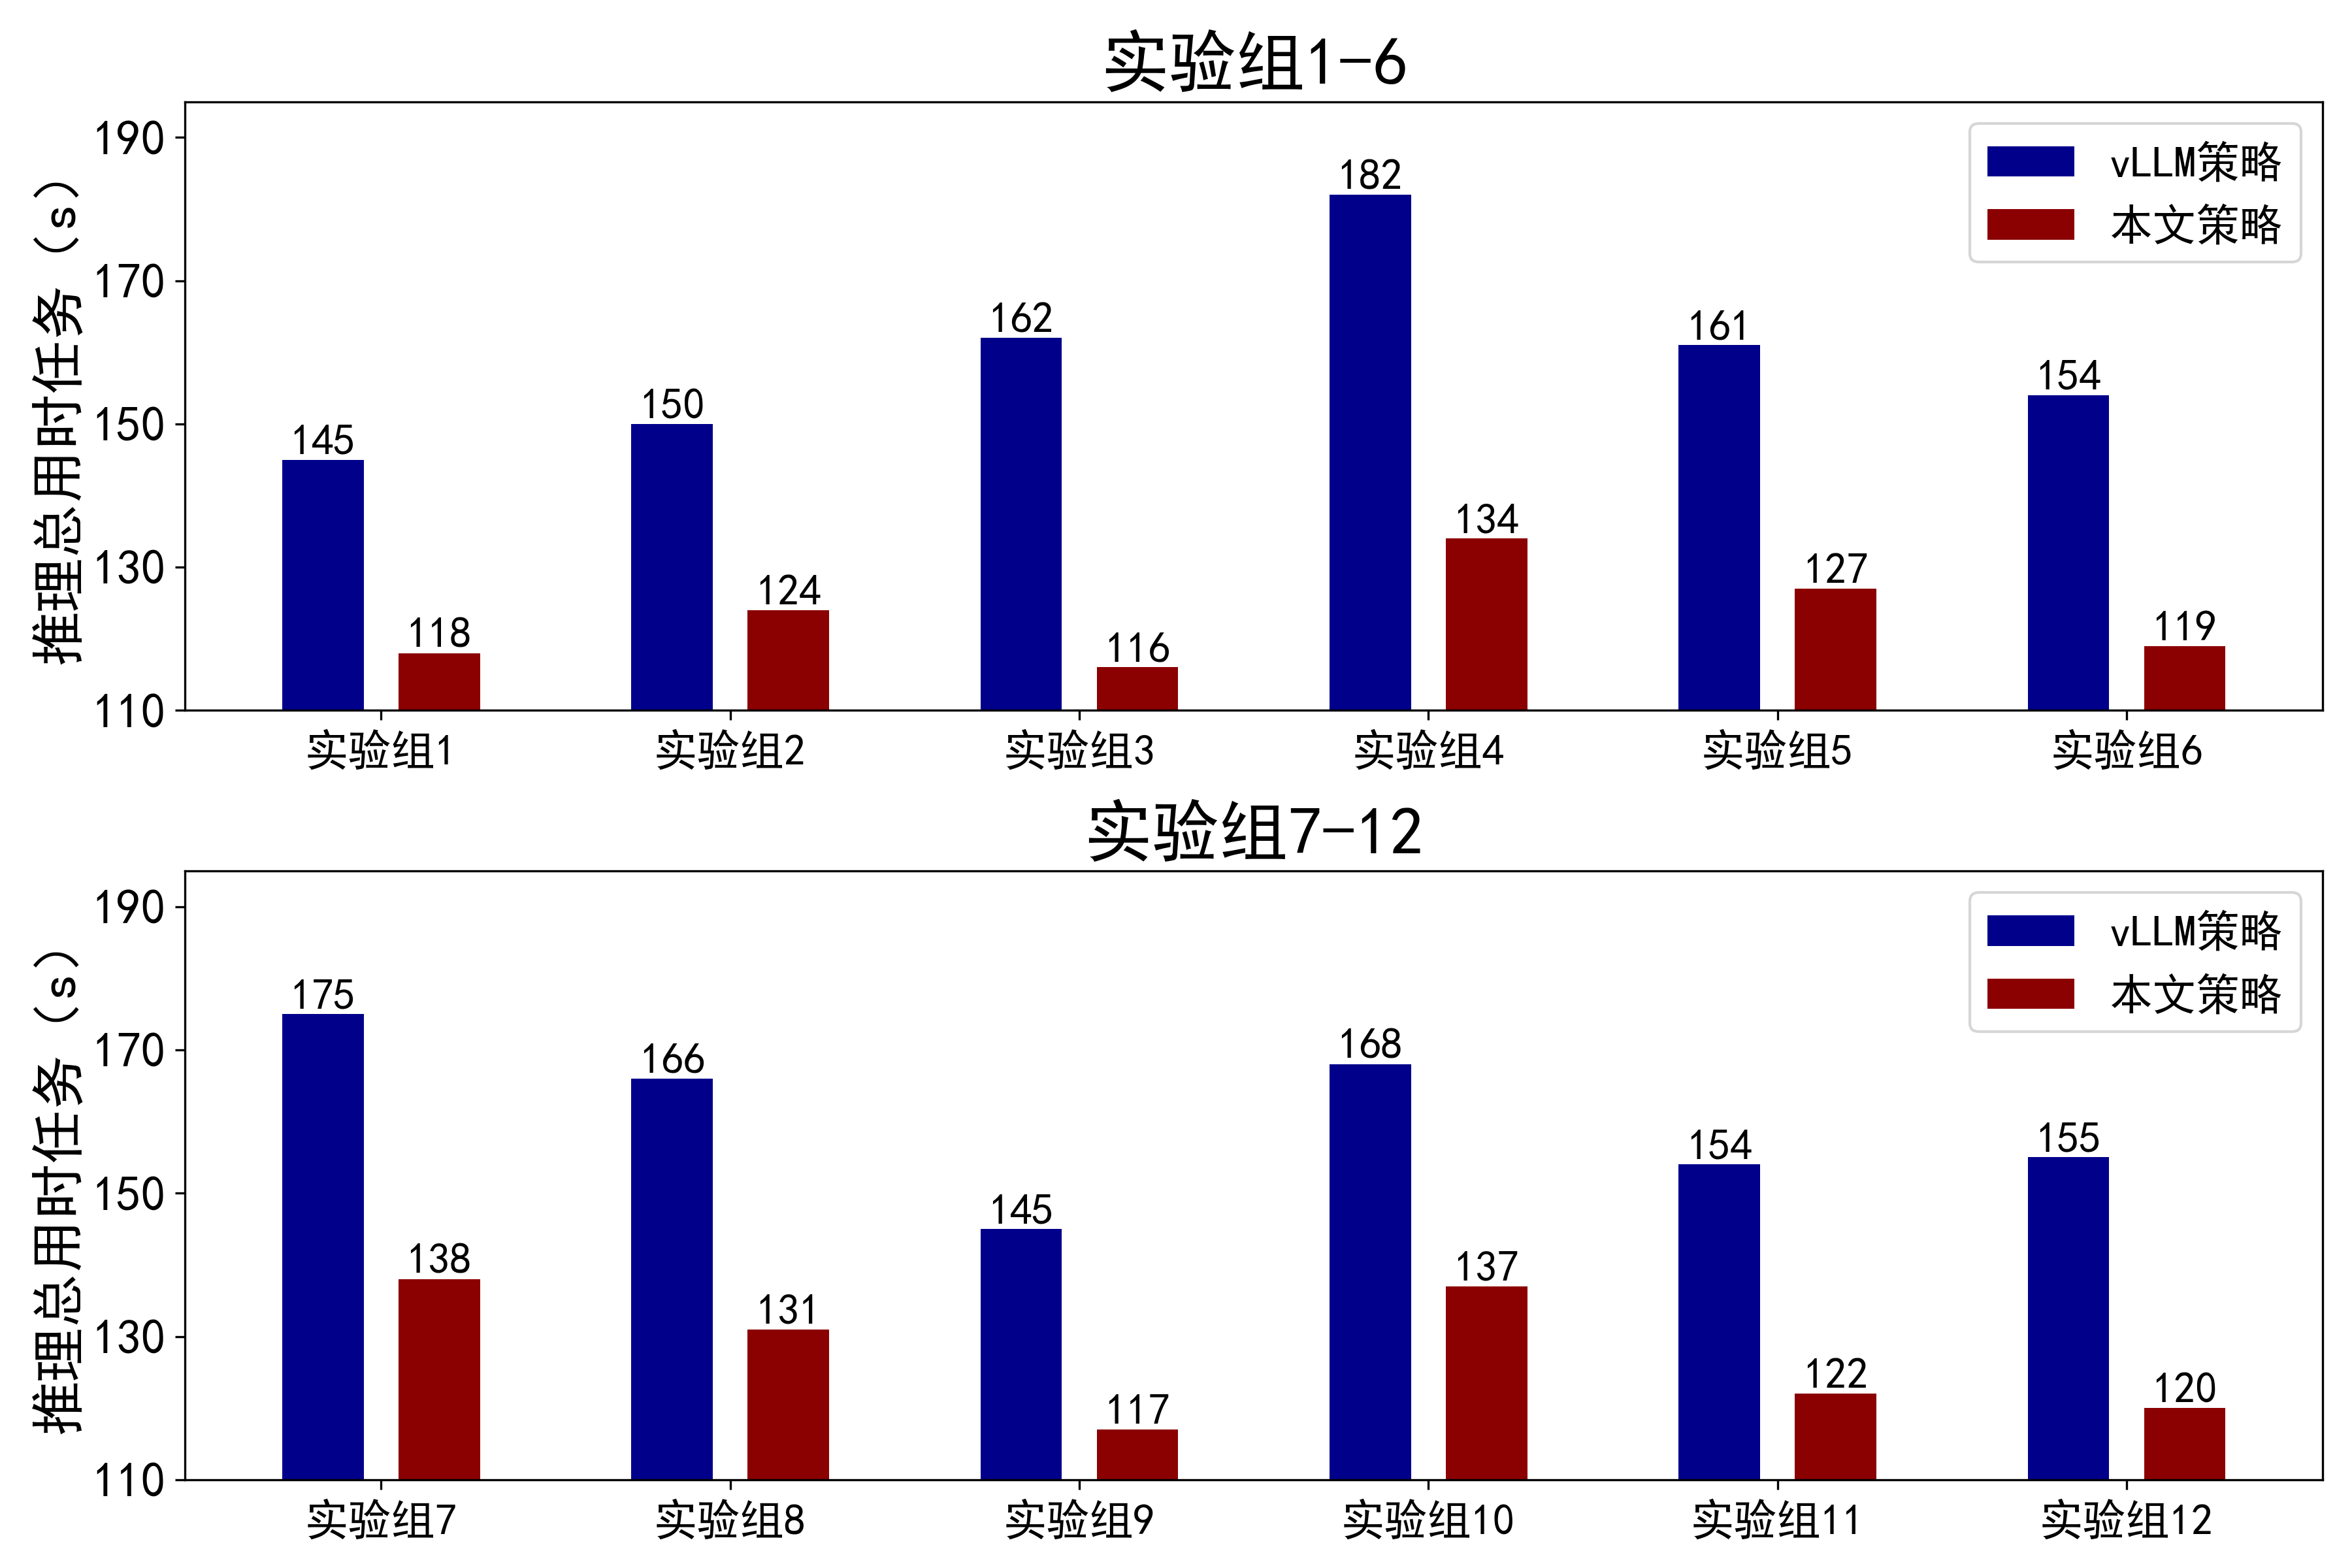
\includegraphics[width=1\linewidth]
  {推理任务总用时.png}
  \caption{推理任务总用时}
  \label{推理任务总用时}
\end{figure}

\begin{figure}[!htbp]
  \centering
  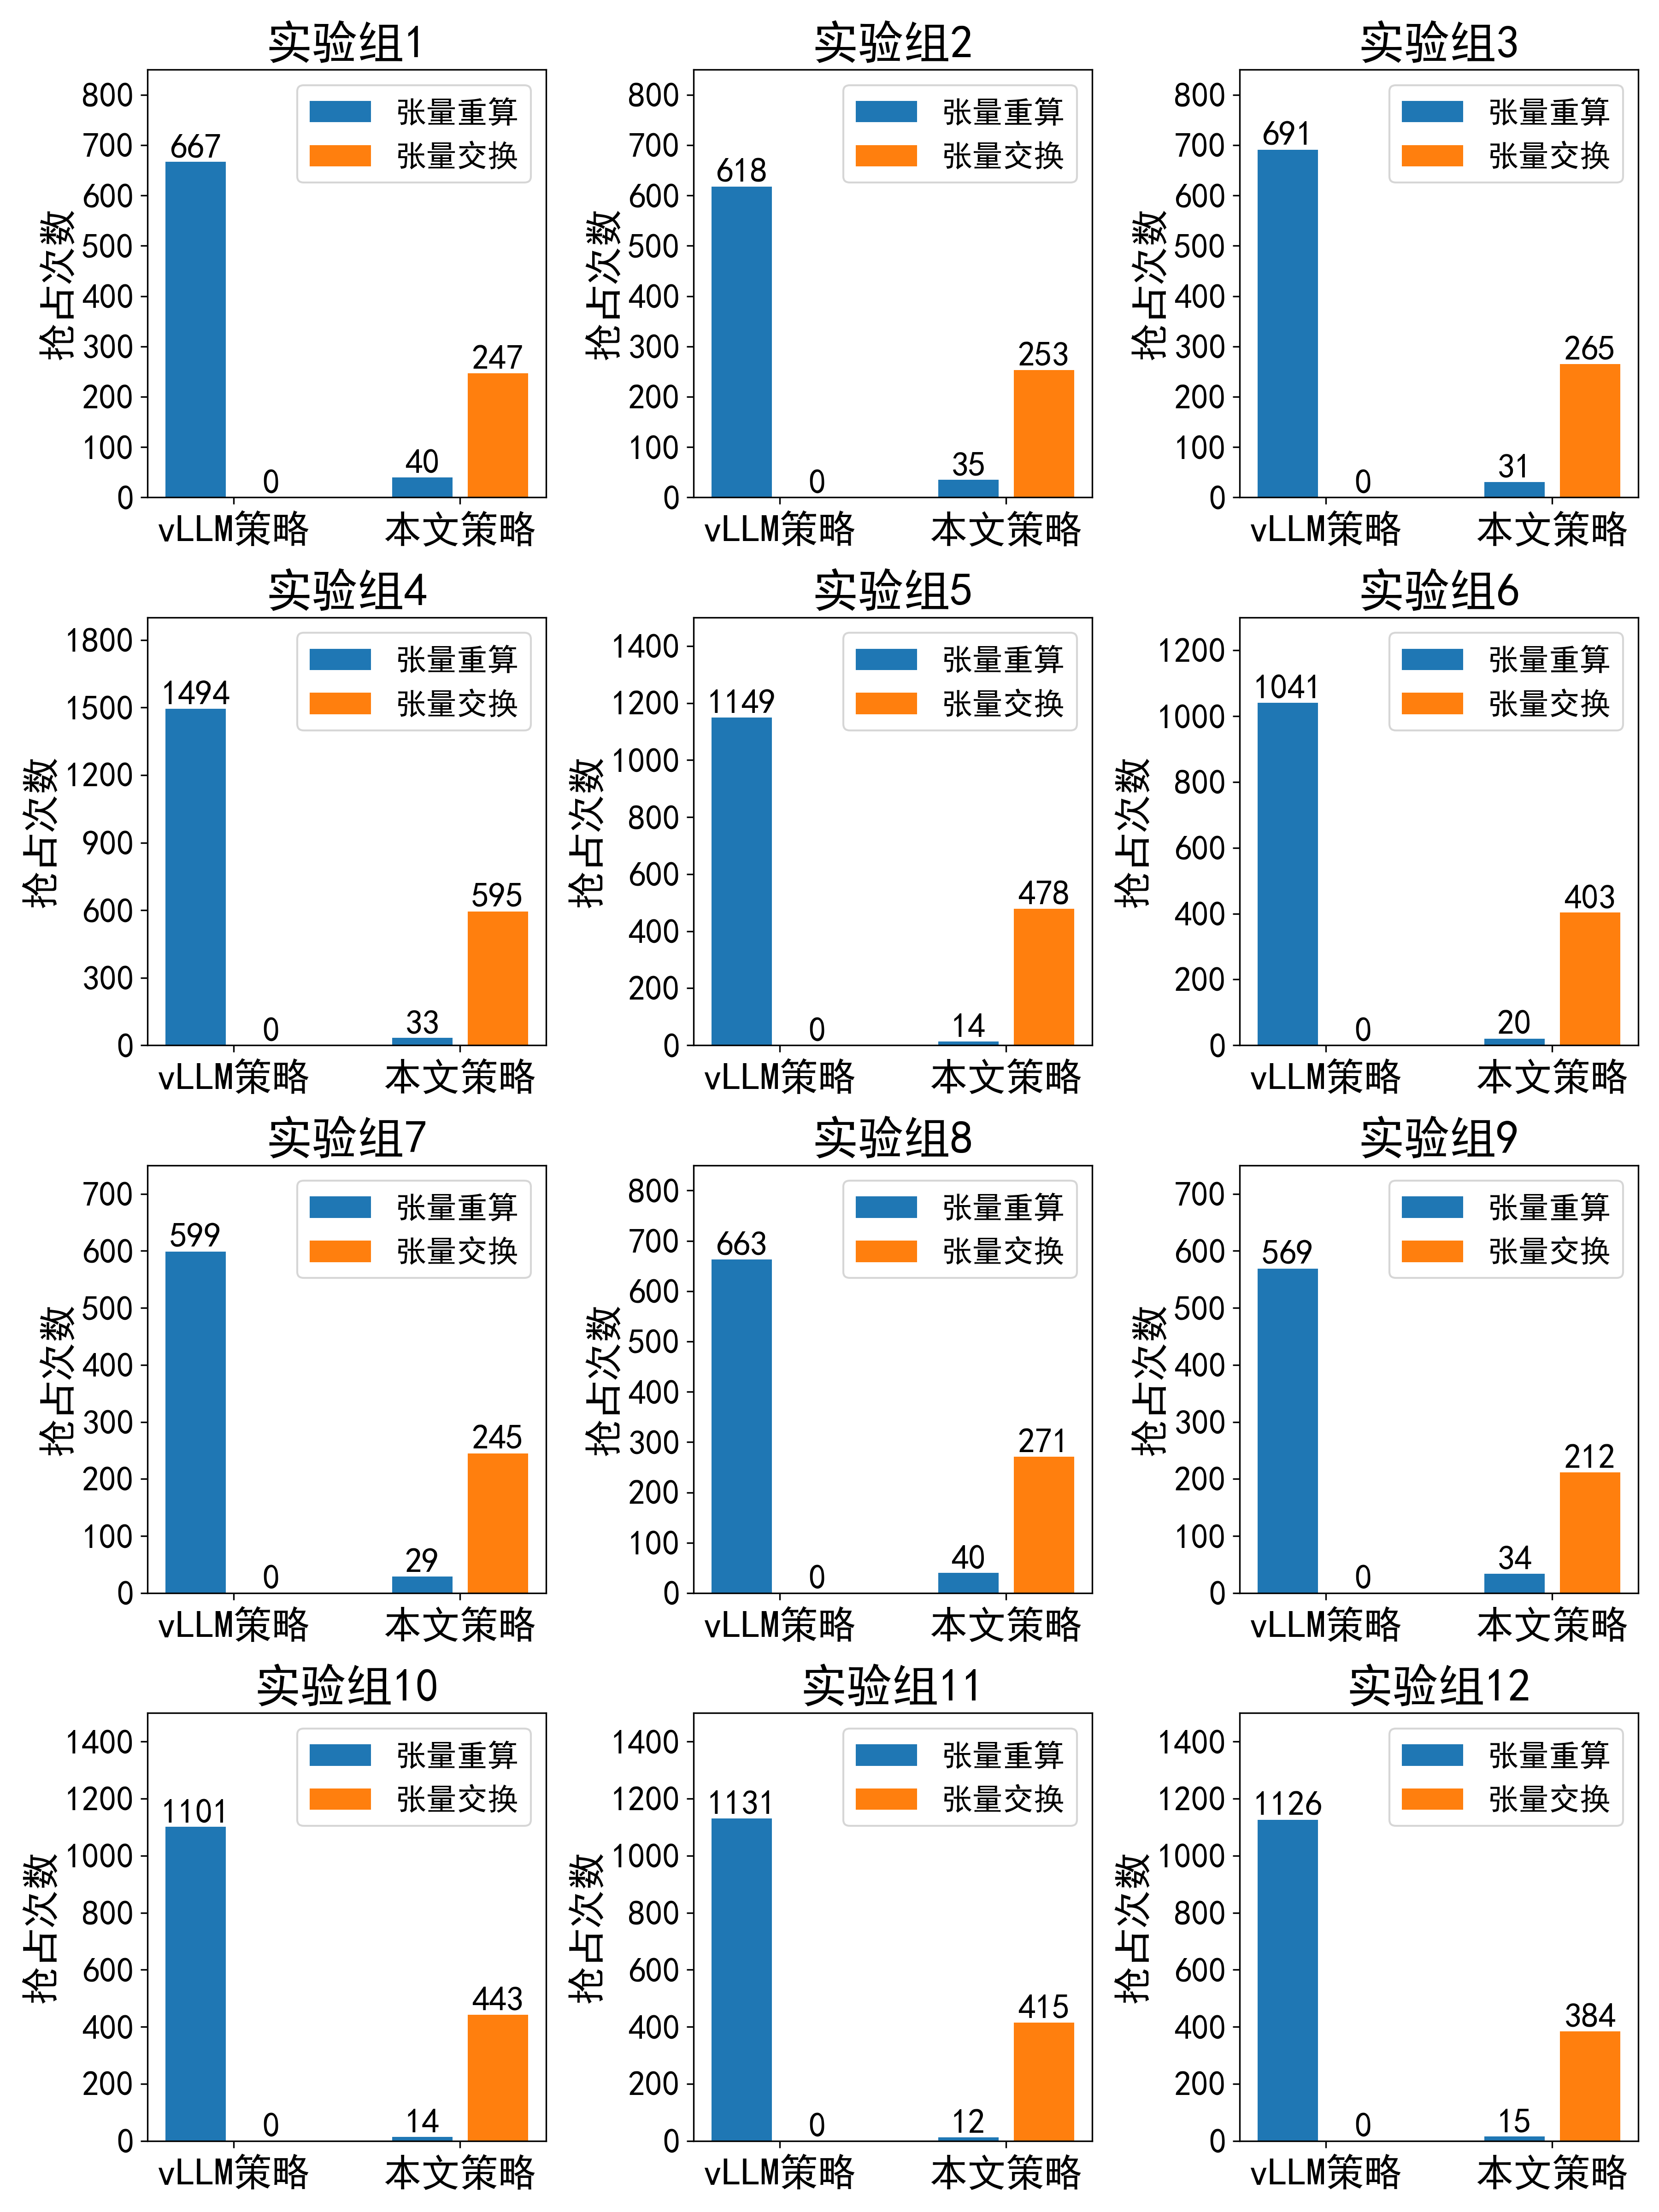
\includegraphics[width=1\linewidth]
  {用户请求抢占次数.png}
  \caption{用户请求抢占次数}
  \label{用户请求抢占次数}
\end{figure}

\subsection{实时性测试}
为了消除整体吞吐率变化对实时性测试的影响,本文选取平均带权周转时间作为测试指标。用户请求带权周转时间等于客户端响应时间除以服务器端处理时间,如公式\ref{Weighted Around Time}所示。该指标越低,说明用户请求的排队时间越短。 \par
\begin{equation}
  \begin{aligned}
    weighted\_around\_time = \\ \frac{finish\_time - recieve\_time}{finish\_time - schedule\_time}
  \end{aligned}
  \label{Weighted Around Time}
\end{equation}

\begin{table}[H]
  \centering
  \caption{本文策略在12个实验组中的加速比}
  \label{本文策略在12个实验组中的加速比}
  \small
  \begin{tabular}{|c|c|c|c|c|c|c|}
    \hline
    \textbf{实验组} & \textbf{1} & \textbf{2} & \textbf{3} & \textbf{4} & \textbf{5} & \textbf{6} \\ \hline
    \textbf{整体加速比} & 1.23 & 1.21 & 1.40 & 1.36 & 1.27 & 1.29 \\ \hline
    \textbf{实验组} & \textbf{7} & \textbf{8} & \textbf{9} & \textbf{10} & \textbf{11} & \textbf{12} \\ \hline
    \textbf{整体加速比} & 1.27 & 1.27 & 1.24 & 1.23 & 1.26 & 1.29 \\ \hline
  \end{tabular}
\end{table}

图\ref{用户请求平均带权周转时间}展示了本实验的测试结果。由图可知,本文策略使得用户请求的平均带权周转时间显著下降,说明用户请求从客户端发送至服务器端后能够很快开始处理,不会出现长时间等待现象。
\begin{figure}[!htbp]
  \centering
  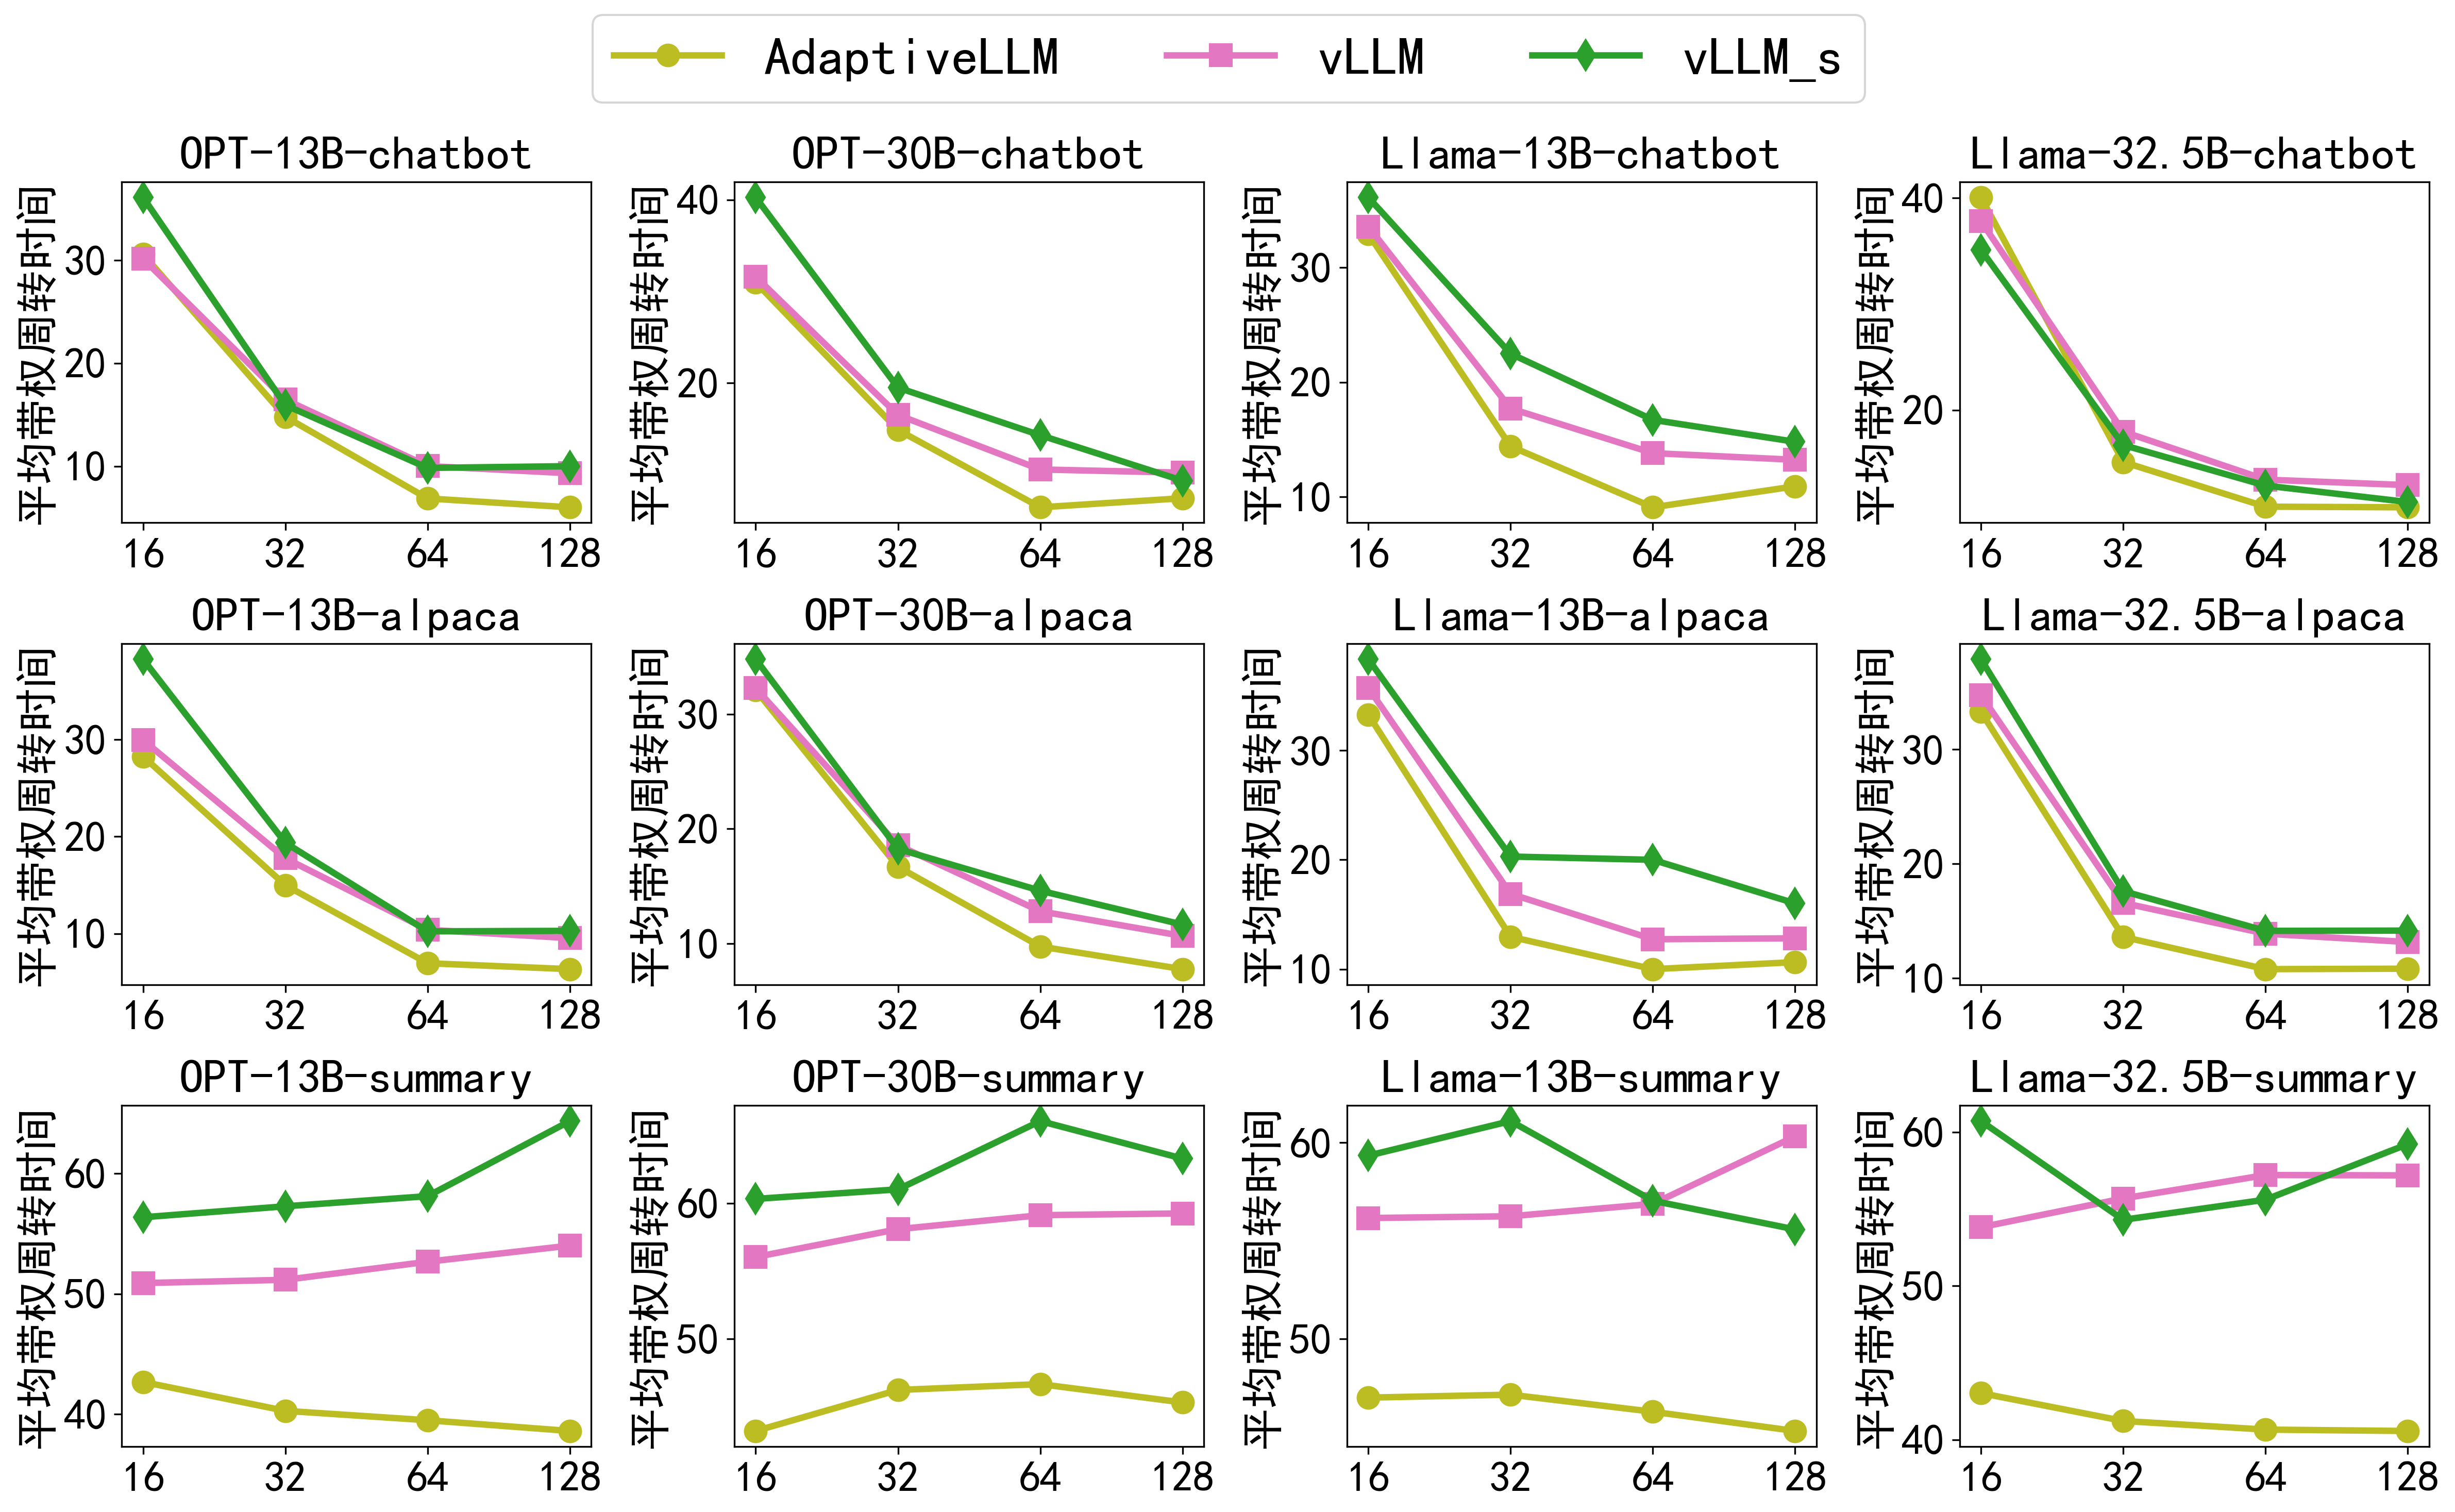
\includegraphics[width=1\linewidth]
  {用户请求平均带权周转时间.png}
  \caption{用户请求平均带权周转时间}
  \label{用户请求平均带权周转时间}
\end{figure}

\subsection{其它测试}
\subsubsection{误差分析}
张量重算(单次prefill阶段执行)开销的预测误差等于单步推理执行时间预测器的误差,根据本章第三节的分析可知,其预测误差低于2\%。 \par
本文针对实验组1和4进行交换误差测试,其结果如图\ref{交换开销预测误差}所示。在这两个实验组中,换出开销预测MAPE误差分别为0.4\%和2.3\%;换入开销预测MAPE误差分别为1.3\%和1.4\%。因此,张量交换开销的计算误差低于5\%。
\begin{figure}[!htbp]
  \centering
  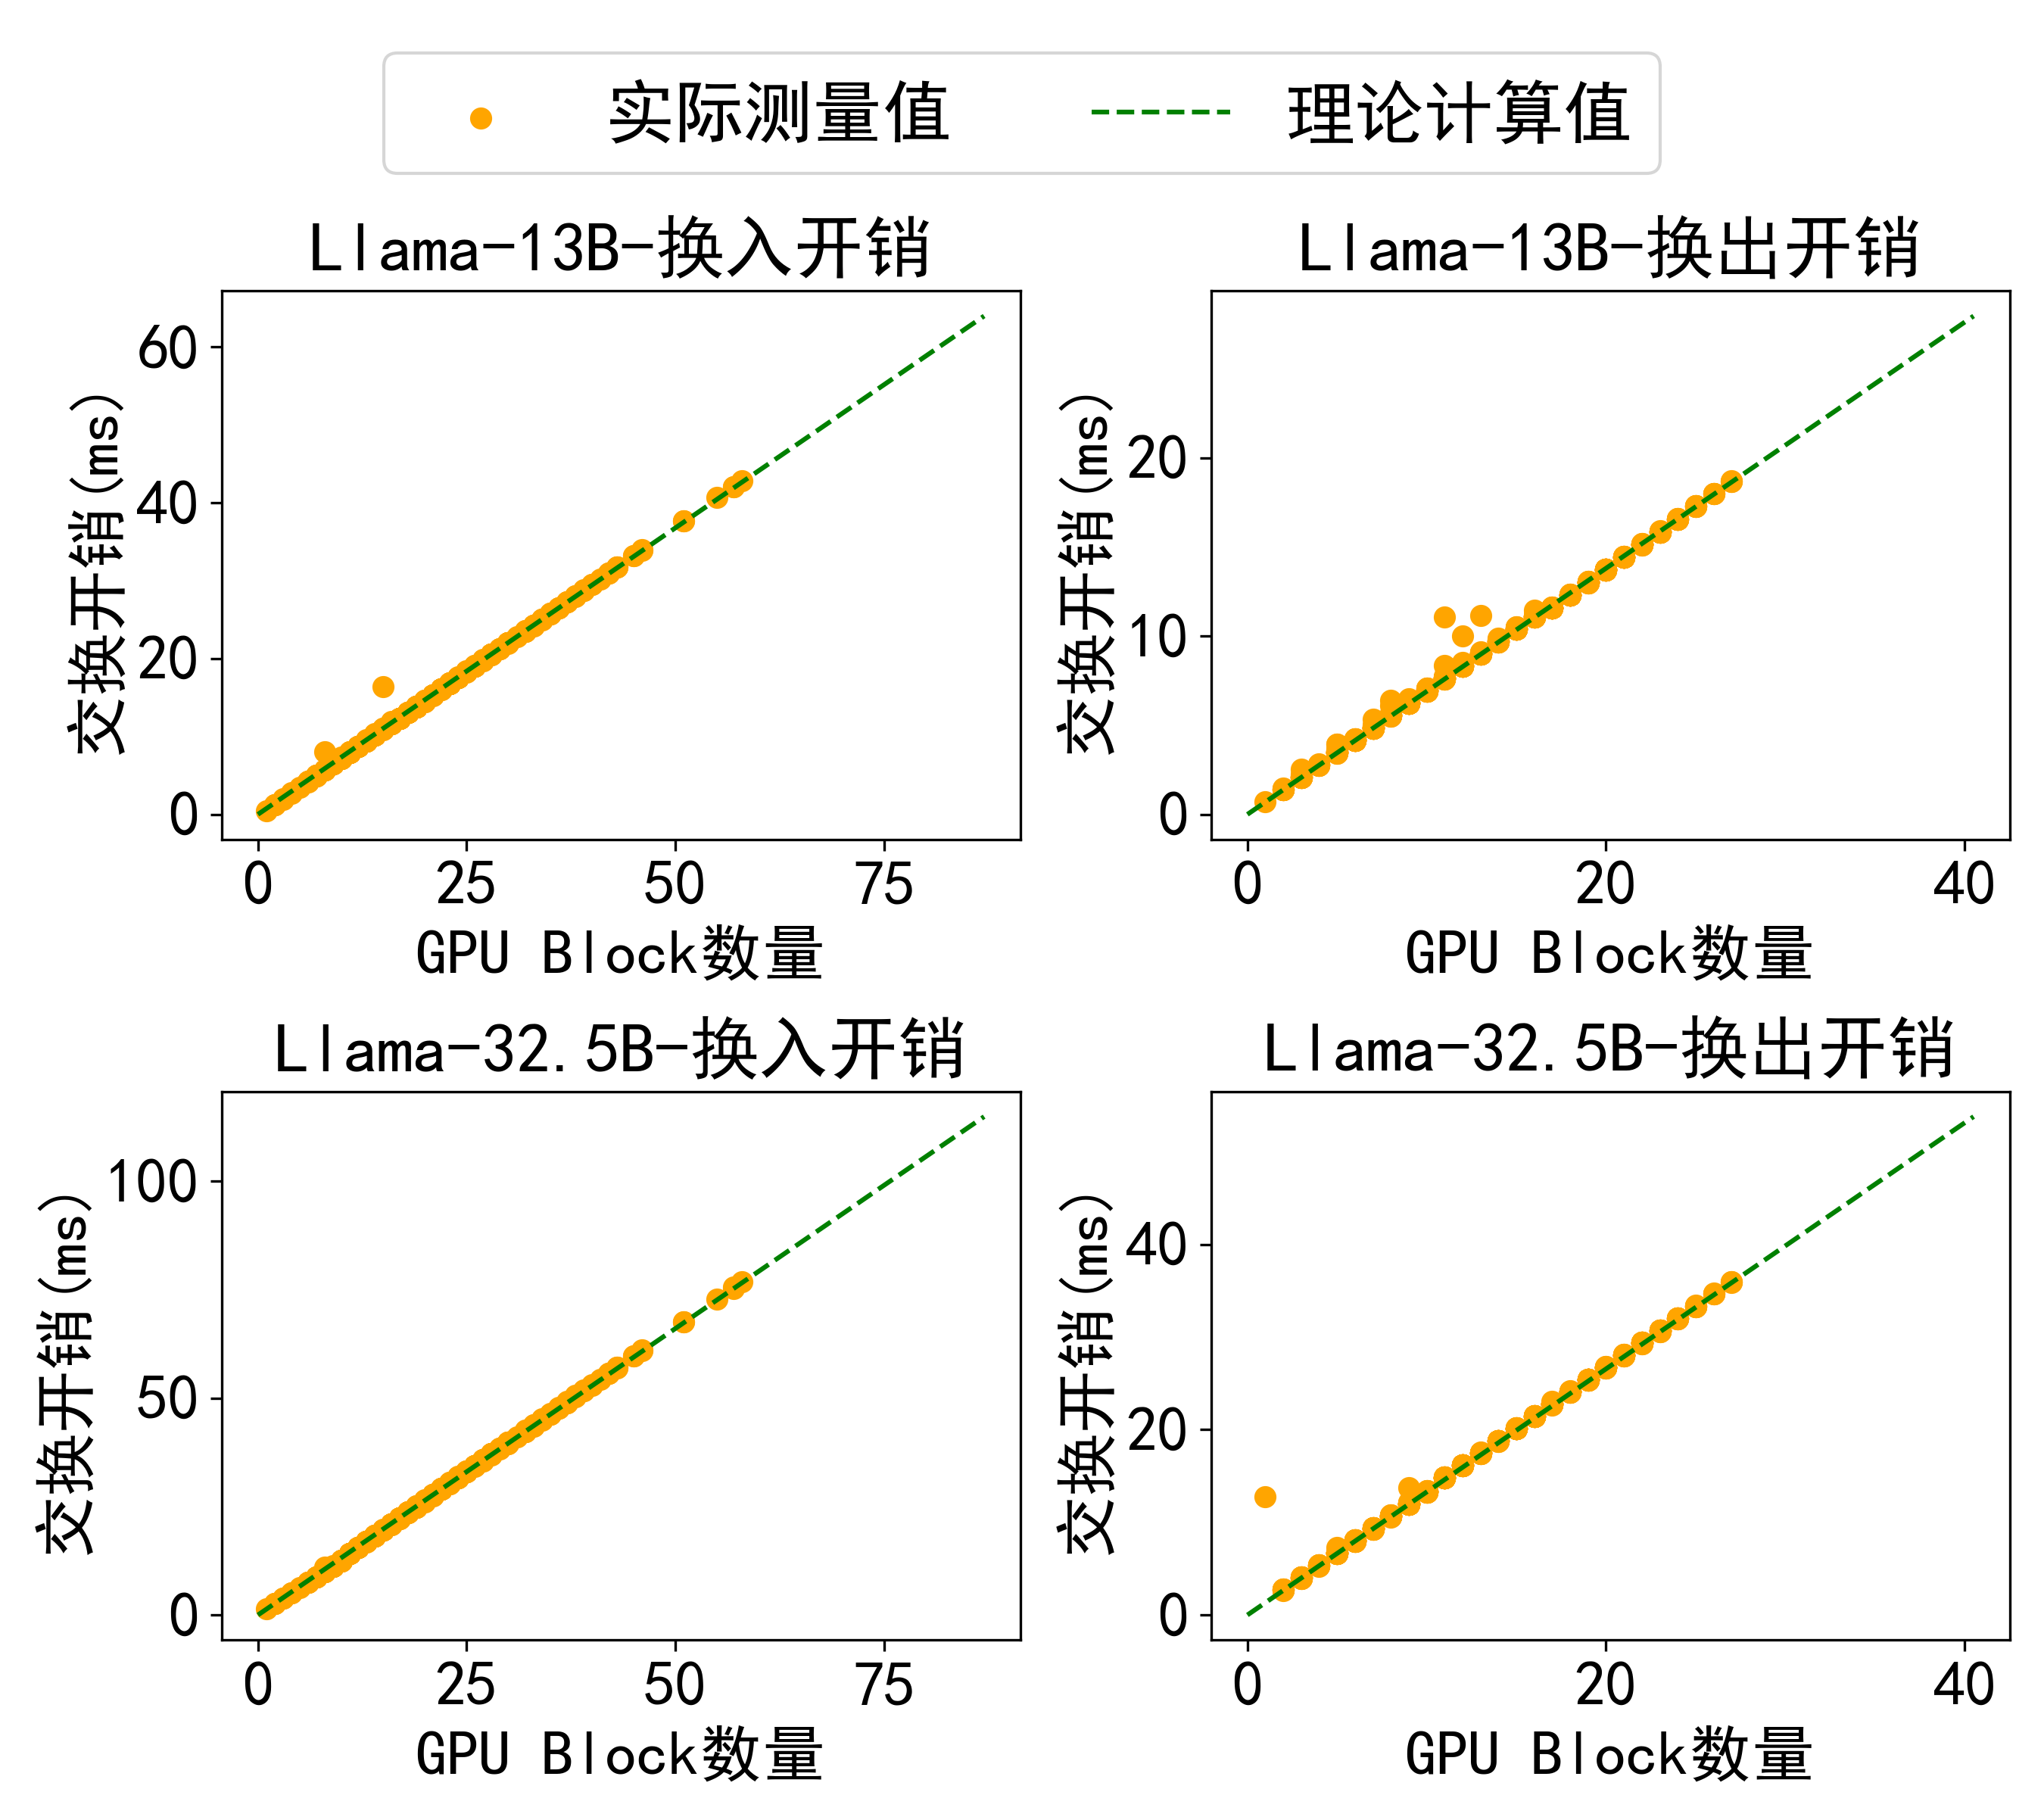
\includegraphics[width=0.9\linewidth]
  {交换开销预测误差.png}
  \caption{交换开销预测误差}
  \label{交换开销预测误差}
\end{figure}

\subsubsection{开销分析}
基于开销感知的张量优化策略在获取重算和交换开销时,会带来新的预测开销。本文设计如下对照实验获取张量感知过程的开销: \par
在吞吐率测试过程中,当GPU内存不足时调用开销比较过程,但最终使用vLLM提供的固定式张量抢占策略(重算)。观察此情景下推理任务的总用时可知,张量感知过程的开销在整个推理任务中仅占1\%至2\%。
    
\section{结论}
本文设计了一款基于张量交换和张量重算的LLM推理服务框架。首先,实现了张量重算开销预测与张量交换开销预测,其预测误差分别在2\%和5\%以下。其次,引入了基于开销感知的张量优化策略和基于公平性的用户请求调度策略。基于开销感知的张量优化策略用于在GPU内存不足时选择开销较小的抢占方式,减小抢占开销。实验表明,该策略为推理任务带来20\%-40\%的整体吞吐率提升,实现了服务器端的处理加速。基于公平性的用户请求调度策略能够以合理的方式调度所有用户请求,减少其等待时间,实现了面向客户端的实时请求处理。本文实现了整体吞吐率与单请求延时的权衡,化解了二者在优化实现上的矛盾。
    
\end{document}


